\chapter{HIV Neutralizing Antibodies in HIV Na\"{i}ve Donors}
\section{Introduction}
The induction of broadly neutralizing HIV-specific antibodies is likely to be a critical component of the mechanisms of protection for an effective HIV vaccine. In the work presented here, we used a novel approach for examining the heavy chain complimentary determining region 3 (HCDR3) repertoire of HIV-naïve donors to interrogate the structural properties of long HCDR3 loops. Some broadly neutralizing HIV-neutralizing human antibodies possess long HCDR3 regions, which typically are created at the time of original antibody gene recombination rather than during somatic hypermutation. We sought to determine if antibodies with long, structured HCDR3s that are present in the naïve B-cell repertoire of HIV-naïve donors confer neutralizing properties to those antibodies similar to that of previously isolated HIV-neutralizing antibodies such as PG9 and PG16, which target the HIV envelope protein variable loops 1 and 2. Using ultra-deep nucleotide sequence analysis of HCDR3 regions in antibody gene replicons for 64 different HIV-naïve donors, we obtained approximately 25,000 unique sequences that encoded HCDR3s of 30 amino acids in length. The modeling suite Rosetta was used to assess the ability of these 30 amino acid length HCDR3 sequences to form a loop with structure similar that of antibody PG9. The PG9 backbone template then was threaded rapidly with sequences from HIV-naïve donors to evaluate the energetic state of naturally occurring long HCDR3s when tested in a PG9-like conformation. The sequences encoding HCDR3s with the most favorable predicted energy states in this conformation then were redesigned in silico to optimize binding with minimal changes, simulating the process of somatic hypermutation. The sequences that were found to mimic the binding energy and HCDR3 structure of PG9 were synthesized and characterized experimentally for ability to bind to HIV envelope (env) protein and neutralize HIV infectious virions. We find 12 unique antibodies that present PG9 HCDR3 mimicry with 0 to 7 mutations away from their respective HIV-naïve wild-type sequence. This work, using a robust new bioinformatics and modeling pipeline, suggests that HIV-naïve donors may possess naïve B-cells encoding antibodies with long HCDR3s that can neutralize HIV prior to infection. Expanding and preserving these unique naïve B-cells from the naïve repertoire may represent an important new strategy for HIV vaccine priming.

\subsection{Potential Paradigm Shifts in Vaccinology}
Elicitation of broadly neutralizing antibodies (bNAbs) against human immunodeficiency virus type 1 (HIV-1) has been one of the greatest challenges in modern vaccinology1,2. A bNAb response occurs in 10-30\% of those infected, with about 1\% of those possessing ‘elite neutralization’ breadth3. These antibodies typically arise 1 year after infection at the earliest and peak at approximately 3-4 years after infection4. Recent advances in donor selection from cohorts of chronically infected patients, novel screening methods, and antibody isolation technologies, have allowed identification of dozens of new antibodies to the envelope protein gp120/gp41 of HIV-15. These antibodies bind at least five major epitopes on gp120 including the CD4 binding site6, the gp120 outer domain7,  the V3 loop and V3 complex glycans8, the V1/V2 loop and surrounding glycans9, or the membrane proximal region (MPER) on gp4110. While the various bNAbs of interest were isolated using different strategies, they often share certain unusual and distinctive genetic features, such as very large numbers of somatic mutations or very long non-canonical heavy chain complimentary determining region 3 (HCDR3) structures11.

Although studies based on bNAb isolation have revealed new targets for immunogen design and have been useful for experimental therapeutic efficacy12, the design of a vaccine against HIV-1 that induces sterilizing or protective immunity has remained elusive13. For example, the RV144 trial that tested a vaccine strategy using priming immunization with a recombinant canarypox vector followed by a bivalent gp120 protein boosting immunization revealed 31\% efficacy and 60\% efficacy in the first year for this regimen14. While the RV144 trial results did suggest modest efficacy, the waning of protection after one year suggested major improvement in immunogenicity is still needed. An obstacle in vaccine development for elicitation of bNAbs is the limited understanding of the maturation process from germline to hypermutated variable gene segments or the process for eliciting secretion of antibodies with long HCDR3s, which are characteristic of a number of mature bNAbs15.

One recent study conducted by Doria-Rose and colleagues at the Vaccine Research Center (VRC) structurally characterized twelve somatically related V1/V2 binders that share characteristics with PG9 and PG16 including a long protruding HCDR3 loop that are tyrosine sulfated16. They found that the unmutated common ancestor was found at 30-38 weeks post infection and was able to weakly neutralize superinfecting virus. This finding is a great step in corroborating our rationale for eliciting these types of V1/V2 binders as a strategy for vaccine development.

Here, we attempted to study the occurrence of antibodies in the naïve B-cell repertoire with long HCDR3s that might mediate neutralization of HIV, prior to exposure to HIV antigens. We examined the HCDR3 repertoire of a large number of HIV-naïve donors in context of the HCDR3 structure of the V2/V3-binding antibody PG9. This antibody was isolated initially from the IAVI African Protocol G cohort using high-throughput B cell microneutralization assays to identify functional B cell clones9. These antibodies possess unusual HCDR3 structures characterized by a 30 amino acid long (IMGT numbering) hammerhead-structured HCDR3 region that protrudes about 20Å from the surface of the rest of the combining site17,18. Initial studies using point mutations identified the HCDR3 as the primary structural feature that mediated neutralization17, and this finding was confirmed later by atomic-resolution structural studies of the mAbs in complex with V1/V2 scaffolds19,20.Using ultra-deep sequencing technology along with a robust molecular modeling pipeline, we identified long HCDR3 sequences from the B-cells of HIV-naïve donors that were predicted to mimic the unusual structure of mAb PG9. First, we identified 30 amino

\subsection{Ultra High-Throughput Sequencing}
Through the remainder of this section I will refer to next-generation sequencing as high-throughput sequencing (HTS). This includes Roche© 454-pyrosequencing, Illumina MiSeq©, IonTorrent©, and PacBio© platforms. These high-throughput sequencing technologies tend to give longer read lengths and sacrifice throughput from 0.7 to 95 gigabases (figure \ref{fig:figure3_1} and table \ref{tab:table3_1}) 24.

In contrast, some platforms fall into what I call ultra high-throughput sequencing, including those of the Illumina HiSeq© and SoLiD© platform which sacrifices shorter reads for higher throughput from 320-600 gigabases (figure \ref{fig:figure3_1}, table \ref{tab:table3_1})24. The advances in HTS spurred an initial investigation to examine the healthy donor repertoire in our laboratory.

\begin{figure}
   \centering
   \includegraphics[scale=.5]{images/chapter3/figure3_1.pdf} % requires the graphicx package
   \caption[Current Sequencing Technologies]{Current sequencing technologies. On the x-axis is the current read length for each sequencing platform. The y-axis is the bases per run. Each point is a new iteration of that platforms sequencing read length and coverage. HiSeq has the most coverage with relatively short read lengths. Figure adapted from \citep{developmentinNGS:2012bs} }
   \label{fig:figure3_1}
\end{figure}
\begin{table}
\centering
\resizebox{.99\linewidth}{!}{
\begin{tabular}{llllcc}
\toprule
\textbf{Platform}   & \textbf{Instrument}      & \textbf{Year} & \textbf{Reads per run} & \textbf{Read length (mode or average)} & \textbf{Bases per run (gigabases)} \\
\midrule
Sanger & 3730xl          & ND   & 96            & 800                           & 0.0000768                 \\
454        & GS20            & 2005 & 200000        & 100                           & 0.02                      \\
454        & GS FLX          & 2007 & 400000        & 250                           & 0.1                       \\
454        & GS FLX Titanium & 2009 & 1000000       & 500                           & 0.45                      \\
454        & GS FLX+         & 2011 & 1000000       & 700                           & 0.7                       \\
454        & GS Junior       & 2010 & 100000        & 400                           & 0.04                      \\
IonTorrent & PGM 314 chip    & 2011 & 100000        & 100                           & 0.01                      \\
IonTorrent & PGM 316 chip    & 2011 & 1000000       & 100                           & 0.1                       \\
IonTorrent & PGM 318 chip    & 2011 & 5000000       & 100                           & 0.5                       \\
IonTorrent & PGM 318 chip    & 2012 & 5000000       & 200                           & 1                         \\
IonTorrent & PGM 318 chip V2 & 2013 & 5000000       & 400                           & 2                         \\
IonTorrent & Proton PI       & 2012 & 50000000      & 200                           & 10                        \\
Illumina   & GA              & 2008 & 28000000      & 35                            & 1                         \\
Illumina   & GA II           & ND   & 100000000     & 50                            & 5                         \\
Illumina   & GAIIx           & 2009 & 440000000     & 75                            & 33                        \\
Illumina   & GAIIx           & 2011 & 640000000     & 75                            & 48                        \\
Illumina   & GAIIx           & 2012 & 640000000     & 150                           & 95                        \\
Illumina   & HiSeq 2000      & 2010 & 2000000000    & 100                           & 200                       \\
Illumina   & HiSeq 2000      & 2011 & 3000000000    & 100                           & 600                       \\
Illumina   & HiSeq 2500 RR   & 2012 & 600000000     & 150                           & 180                       \\
Illumina   & MiSeq           & 2011 & 30000000      & 150                           & 4.5                       \\
Illumina   & MiSeq           & 2012 & 30000000      & 250                           & 8.5                       \\
Illumina   & MiSeq           & 2013 & 30000000      & 300                           & 15                        \\
SOLiD      & 3               & ND   & 320000000     & 50                            & 16                        \\
SOLiD      & 4               & ND   & 2000000000    & 50                            & 100                       \\
SOLiD      & 5500xl          & 2011 & 3000000000    & 60                            & 180                       \\
SOLiD      & 5500xl W        & 2013 & 3000000000    & 75                            & 320                       \\
PacBio     & RS C1           & 2011 & 36000         & 1300                          & 0.045                     \\
PacBio     & RS C2           & 2012 & 36000         & 2500                          & 0.090                     \\
PacBio     & RS C2 XL        & 2012 & 36000         & 4300                          & 0.155                     \\
PacBio     & RS II C2 XL     & 2013 & 47000         & 4600                          & 0.216                    \\
\bottomrule
\end{tabular}}
\caption[Current HTS Sequencing Platforms]{Figure adapted from \citep{developmentinNGS:2012bs}}
\label{tab:table3_1}
\end{table}

\subsection{Long Long HCDR3s are Established at Original Recombination}
Using first generation HTS sequencing technology, we first observed long HCDR3 sequences in the healthy HIV-naïve repertoire25. Although, long HCDR3s were known to exist26-28,they are mostly primarily found in chronically HIV-infected subjects9,29-31. This lead to a multiple hypothesis model about the origin of long HCDR3s in chronically infected patients (figure \ref{fig:figure3_2}). Given that long HCDR3 antibodies against HIV are highly mutated relative to other antibodies, it could be hypothesized that insertions and deletions (indels) due to somatic mutations could be responsible for the ‘elongation’ of a long HCDR3. These antibodies could be elicited by a chronic infection or heterogeneous prime-boost vaccine strategy, both of which will exhibit selective pressure for antibody maturation from germline sequence (figure \ref{fig:figure3_2}). This long HCDR3 origin model was known as the ‘mutation’ model.The alternate hypothesis was that long HCDR3s were established in the bone marrow at the time of original recombination and were found in the circulating repertoire at presumably, low frequency, or were selected against due to known issues associated with autoimmunity32-35. This is known as the ‘original recombination’ model.

These two models for the origin of long HCDR3s were the original focus for this project and are detailed in specific aims of Bryan Briney’s thesis and were tested by comparing immunoglobulin sequence repertoires for long HCDR3s to those of canonical length HCDR3s36. We can test these models based on two main assumptions about antibody maturation process. One, all antibodies are generated in the bone marrow from the germline repertoire and affinity mature in the lymph tissue37,38. Thus, an antibody that is recently recombined in the bone marrow would have fewer mutations than antibodies that have gone through multiple rounds of affinity maturation.  Figure \ref{fig:figure3_4}A top panel shows an analysis of peripheral B cell mean number of mutations as a function of HCDR3 length. Longer HCDR3s tend to have lower levels of somatic mutations. Figure \ref{fig:figure3_3}B top panel specifically shows the correlation for IgM and IgG class types that have undergone positive and negative selection.

The second assumption is that the affinity maturation process is associated with insertion and deletion events that are likely to be caused by somatic hypermutation associated proteins39-41. Figure \ref{fig:figure3_4}A and \ref{fig:figure3_4}B lower panels show a negative correlation to insertion-deletion associated (indel) percentage suggesting further evidence towards the ‘original recombination’ model.Finally, a statistically significant change in long HCDR3 percentage between naïve B-cells and class switched IgM and IgG B-cells indicates that these antibody sequences are present at original recombination and are selected against during maturation.

Although the original goal for the work done by Bryan Briney was to determine the genetic origin of HCDR3s, it confirmed a population, albeit a very small one, of very-long HCDR3 sequences that are the same length as many of the exceptional broadly neutralizing antibodies against HIV-1. This fortuitous conclusion, along with rapidly advancing throughput of HTS technology lead to the experimental rationale.

\begin{figure}[pb]
   \centering
   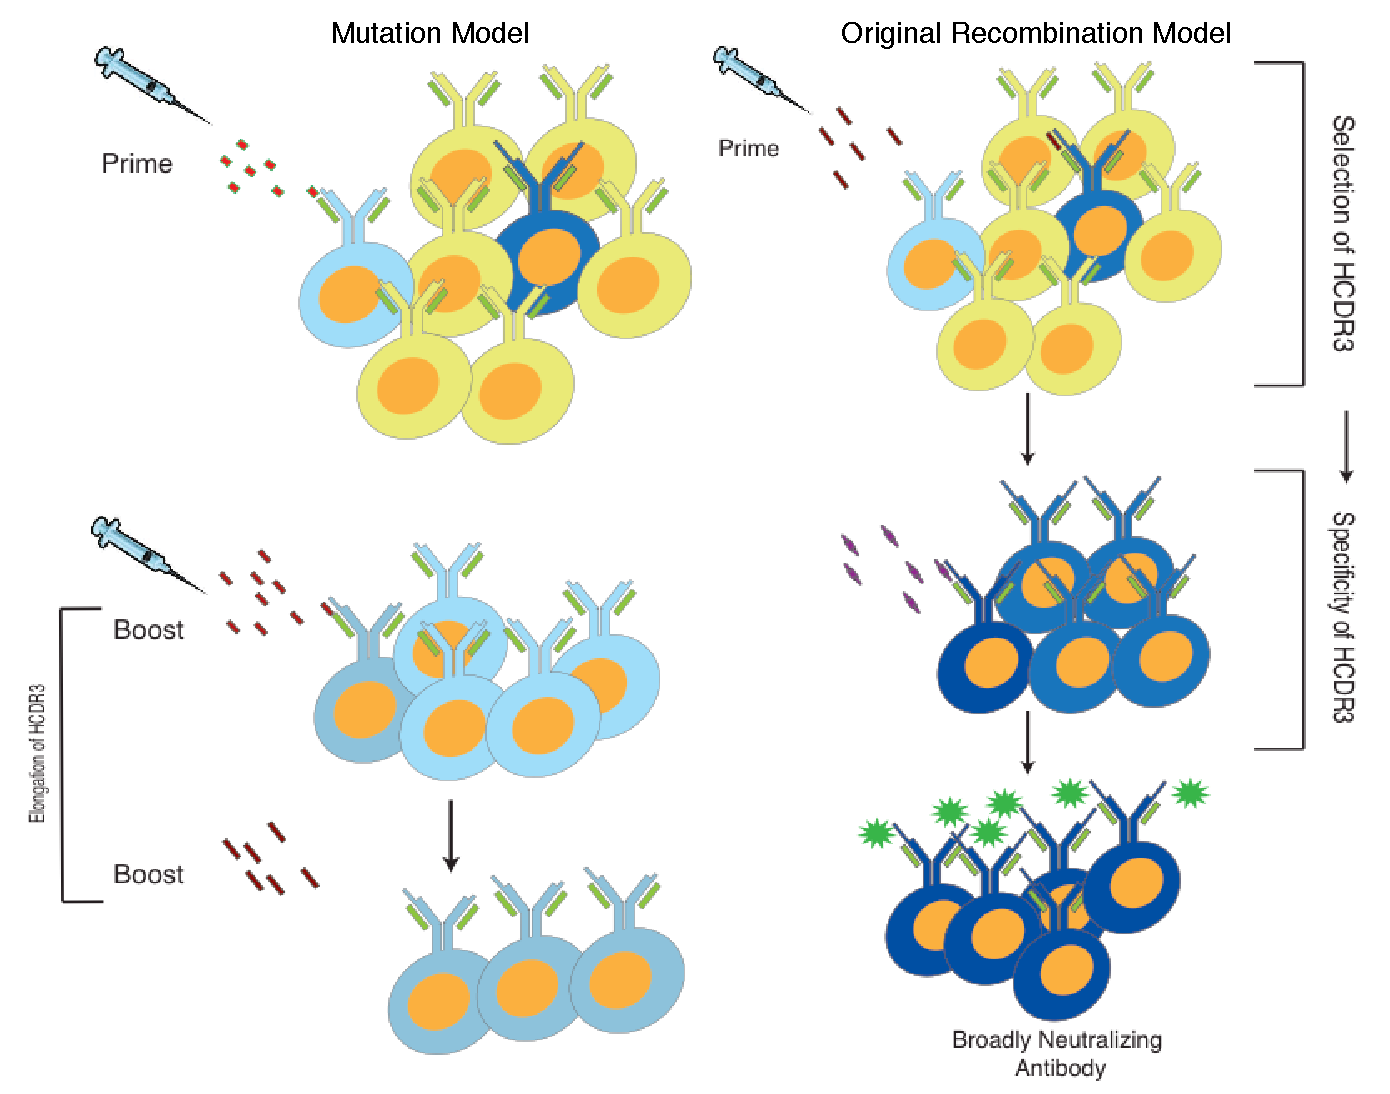
\includegraphics[width=.99\textwidth]{images/chapter3/figure3_2.pdf} % requires the graphicx package
   \caption[Origins of Long HCDR3 Models]{Origins of long HCDR3 models. Two models are proposed to explain the origin of HCDR3s. In the mutation model (left), B-cells (yellow) with canonical length HCDR3s are `elongated' through selective pressure on B-cells (blue) by chronic infection or repeated rounds of vaccine boosts to trigger affinity maturation to an evolving antigen. This repeated round of exposure creates insertions into the long HCDR3. The original recombination model (left) assumes the long HCDR3 is in low frequency in the naive population (yellow). Antigens from a vaccine or chronic infection select the infrequent B cell and expand its clonal population and refine affinity.}
   \label{fig:figure3_2}
\end{figure}

\begin{figure}[t]
   \centering
   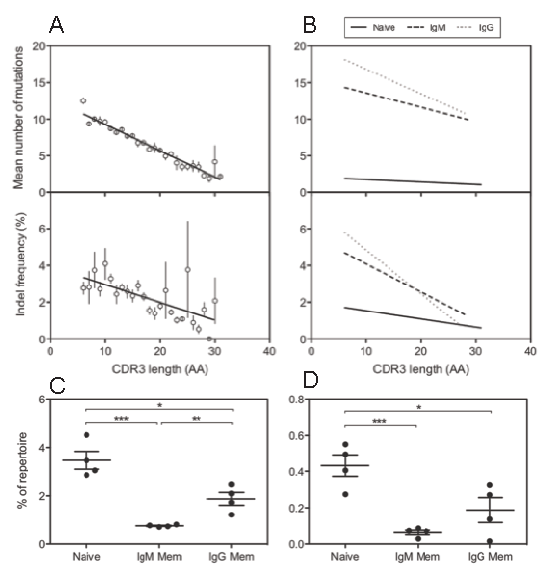
\includegraphics{images/chapter3/figure3_4.pdf} % requires the graphicx package
   \caption[Maturation Sequence Markers and HCDR3 Length]{Maturation Sequence Markers and HCDR3 Length. Insertion and deletion (indel) frequency and mutation frequency is associated as marker for affinity maturation and shows a negative correlation with HCDR3 length (A). The correlation becomes more pronounced in peripheral classed switched B cells IgM and IgG (B). The percentage of the repertoire with long HCDR3s (>24 amino acids, C) and very long HCDR3s (>28 amino acids, D) shows a statistically significant change from naïve B cells to class switched B cells (*** - p < 0.001, * - p < 0.1).}
   \label{fig:figure3_4}
\end{figure}

\subsection{Rationale and Experimental Design}
Our conclusions from examining the HIV naïve repertoire made me question approaches to HIV vaccine design. Traditional reverse vaccinology assumes that we can make a canonical antibody into a broadly neutralizing antibody by a series of prime-boost steps to achieve an optimal level of mutations to produce a protective response to HIV challenge. Indeed, many great strides have been made in the field42. However, the other unique trait about broadly neutralizing antibodies to HIV is many of them possess very long HCDR3s, were almost all of the contact and therefore mechanism of neutralization, stem from the long HCDR31,18,23,43.

With knowledge of the presence of long HCDR3s in HIV naïve donors, and that they are established at the time or recombination, we hypothesized that it was possible for these long HCDR3 sequences to converge on the structural space of some of the long HCDR3 driven broadly neutralizing antibodies. We choose the complex PG9 and a scaffolded epitope V1/V2 to be our template1. The goal was to see if we could mimic the 30-length HCDR3 in PG9 to neutralize HIV (PG9 mimicry). We chose PG9 with the following rationale.

\begin{enumerate}
    \item  The co-crystal structure had recently been elucidated(figure \ref{fig:figure3_3})1.
	\item  The long HCDR3 accounts for neutralization and functionality with few contact residues in other regions of the antibody17,18.
	\item  Germline reversions of the framework still retains neutralization ability12.
	\item  The RV144 trial, the first trial to show substantial vaccine efficacy correlated with an increase in V1/V2 binding antibodies, the binding region of PG944.
	\item  Interactions with the V1/V2 are structure dependent and sequence independent, i.e. backbone-backbone hydrogen bonding across beta-sheets1.
	\item  There is a 9 mutation difference between PG9 and it's sister antibody PG16 at the HCDR3 paratope showing a structural as well as functional convergence irrespective of sequence similarity9,17,18.
\end{enumerate}

The work of Bryan Briney with first generation high-throughput sequencing yielded a low frequency of sequences to test with a length of 30 (0.4\%). Building on this observation, figure \ref{fig:figure3_5} proposes an experimental plan that could test a large number of sequences for PG9 mimicry. In order to make the proposal feasible, we would have to upscale the amount of donors sequenced and the amount of B cell coverage in a new round of next-generation high-throughput sequencing.  We also knew that the coverage necessary was going to produce 500 million to 1 billion sequences, far more data than could be supported on our current architecture.

We planned to implement custom databases and search algorithms to recombine the sequences into a functional antibodyoyme. For prediction of PG9 mimicry, we also needed to develop a structural prediction scheme based on the package Rosetta that would rapidly be able to predict whether a sequence could tolerate the PG9 configuration. We also planned for a tractable amount of recombinant antibodies to be made in the laboratory to test for experimental validation using binding and neutralization analysis.

\begin{figure}
   \centering
   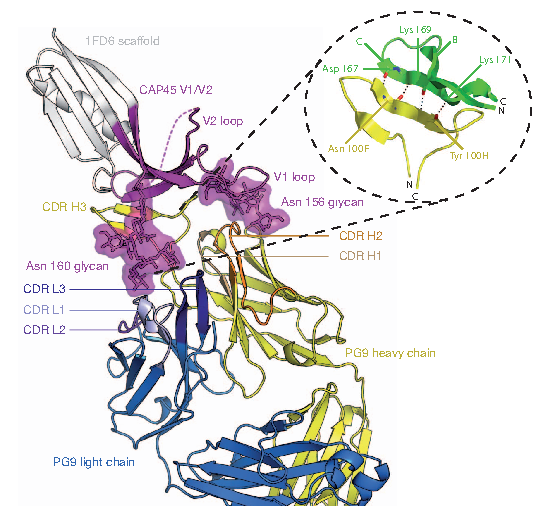
\includegraphics[scale=.8]{images/chapter3/figure3_3.pdf} % requires the graphicx package
   \caption[PG9 Complexed with V1/V2 Scaffold]{PG9 complexed with V1/V2 scaffold. The crystal structure adapted from \citep{McLellan:2011dg}. Beta-sheet interactions at the interface are highlted.}
   \label{fig:figure3_3}
\end{figure}

\begin{figure}
   \centering
   \includegraphics[width=.9\linewidth]{images/chapter3/figure3_5.pdf} % requires the graphicx package
   \caption[Overview of Methodology ]{The methodology can be split into four subsections that are a combination of computational (dashed-line) and experimental work (solid-line). HIV naïve blood is collected from 64 adult donors and the HCDR3 is sequenced on the HiSeq Illumina platform (A). The raw sequences are reconstructed and analyzed against germline databases using custom software. The sequences are parsed and stored in optimized databases to handle the large quantity of antibody sequences (B). HCDR3 sequences are chosen by length and tested for PG9 mimicry using the Rosetta software suite. Iterative rounds of minimization, docking, and design, followed by rigorous statistical analysis allows for a robust prediction of potential candidates from the HIV-naïve repertoire that may neutralize HIV (C). A tractable number of sequences are synthesized and tested experimentally through biophysical characterization and neutralization studies against HIV – 1 (D).}
   \label{fig:figure3_5}
\end{figure}

\section{Ultra High-Throughput Sequencing of HCDR3s}
As explained in the rationale, it was necessary to obtain many more sequences than were available using the coverage of 454-pyrosequencing. We decided to use the HiSeq platform, as the throughput at the time was 109 reads of 150 base pairs (bp). Although, the sequencing read of 150 bp was not long enough to cover the entire antibody variable gene, it would provide coverage of the HCDR3 portion of a recombined gene, sufficient for our experimental goals. We estimated that 0.4\% of the sequences would be greater than 28-length at 3 standard deviations from the mean HCDR3 length. This in theory would afford 400,000 recombined very-long HCDR3 reads.

Using the scheme found in figure \ref{fig:figure3_6}, we indexed 64 different healthy donors with based on a primer design by Bryan Briney and Jessica Finn. First, we obtained 64 HIV-naïve donors through the American Red Cross. No further information was obtained about each donor except for Hepatitis and HIV negative results. The mRNA was purified from the peripheral blood mononuclear cells (PBMC), and subjected to two rounds of PCR. The HiSeq run was done in the VANderibilt Technologies for Advanced GEnomics (VANTAGE). The raw data was reconstructed with paired-end algorithms and run through PyIg (Appendix). This program called on V, D, and J gene segments for the HCDR3 region and stored them to a database custom built for large amounts of information. The statistics for the HiSeq run are found in Table \ref{tab:table3_2}.  The full methodology can be found in the methods appendix section.

Next, we queried our database to get a distribution a frequency of HCDR3 lengths. Without removing any redundancies of amino acid sequences, we binned each length and got a distribution, referred to as all sequences (figure \ref{fig:figure3_7}A). We then removed all redundancies within each donor and plotted them as a function of length, referred to as donor unique (figure \ref{fig:figure3_7}A, B). Finally, we made a distribution that pooled all the sequences together and removed all HCDR3 redundancies, referred to as total unique (figure \ref{fig:figure3_7}A-C). The redundancies found in all donors combined subtracted by all unique sequences are by definition shared in at least one or more donor. For example, for length of HCDR3 equal to 1, we have 174 occurrences when we add up donor unique. That is, for donor 1 we have x amount of unique sequences among that donor added to x amount of sequences for donor 2 and etc. However, when we pool all the sequences of length 1 first, and then remove redundancies, we arrive at 17 unique sequences. That means there are 137 shared amino acid sequences found in one or more donors. An easier way to view it, is to plot the percentage of sequences at a given length that are shared among one or more donor (figure \ref{fig:figure3_7}D). This can actually be done with database queries that are detailed in the appendix.

The mean length of HCDR3 sequences in our dataset was 16.40 \pm 4.03. This was in previous agreement with our work using a much smaller dataset25. Although there is no standard definition of a `'long HCDR3' we arbitrarily chose the cutoff to be two and three standard deviations from the mean for long and very long HCDR3s respectively (24AA, 28AA, Figure \ref{fig:figure3_7}C).Our recombination software (PyIg) can also assign V, D, and J gene families using the BLAST algorithm45. We observed similar trends in D and J gene family usage as a function of length. DH3 and JH6 family increased as length of HCDR3 increased (figure \ref{fig:figure3_7}F, G). This makes intuitive sense these are the longest gene segments in their respective segment. For V-gene families, we did not observe a different in germline gene usage as a function of length (figure \ref{fig:figure3_7}E). This trend was also reported with our previous work in which we sequenced the entire antibody segment, however, we can’t be absolutely confident in our assignments of V-gene considering we only have on average a 20 bp overlap. We can also narrow down individual genes for the D-gene segment and observed an increase in DH2-2, DH2-15, DH3-3, DH3-10 and DH3-22 as HCDR3 length increased (figure 3.7H).  With a full dataset, we were ready to begin predictions for long HCDR3s that can mimic PG9 using the Rosetta software suite.

\begin{figure}
   \centering
   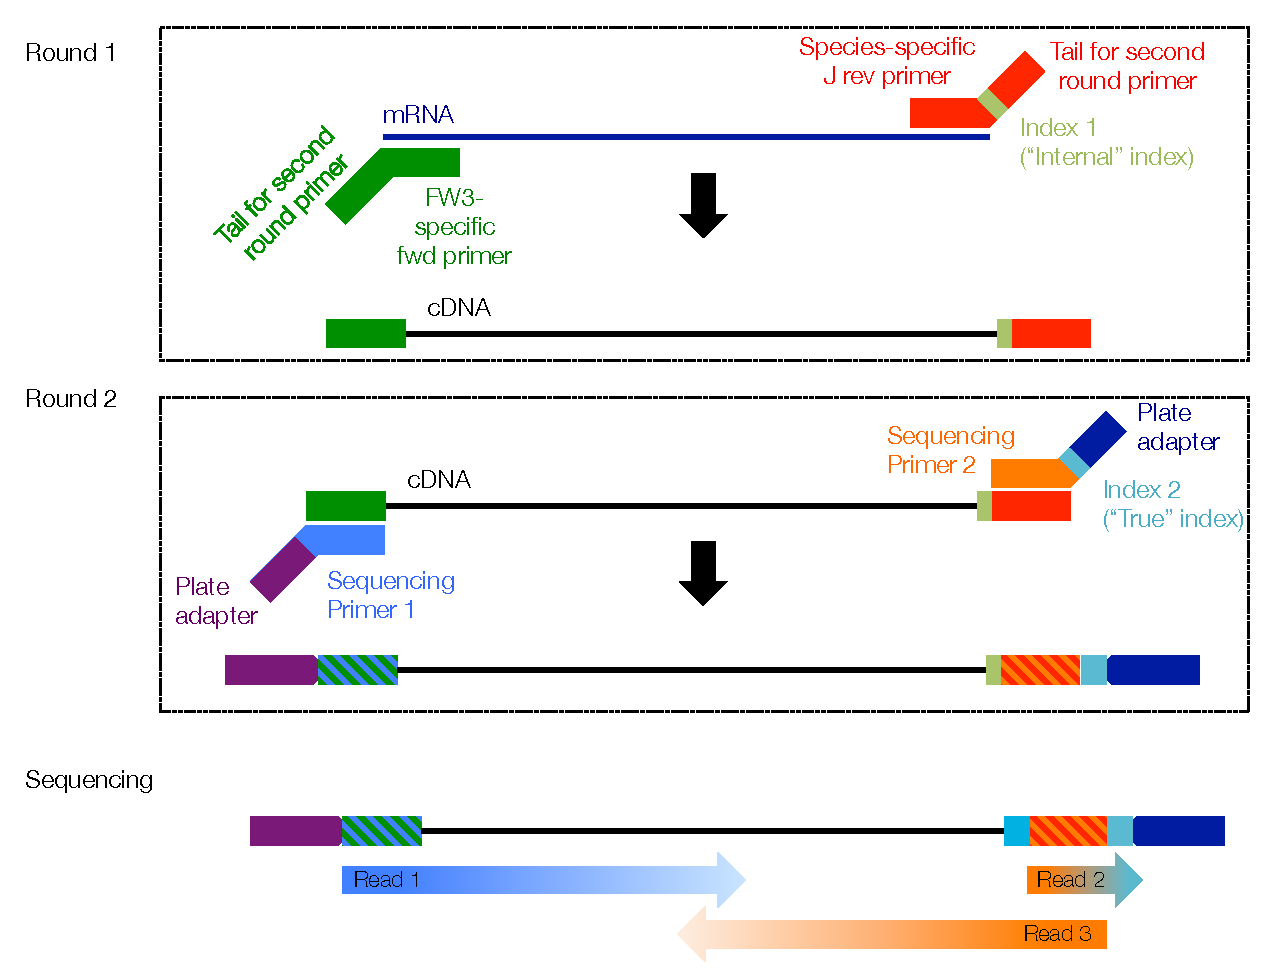
\includegraphics[width=.9\linewidth]{images/chapter3/figure3_6.pdf} % requires the graphicx package
   \caption[Overview of HiSeq Scheme]{RT-PCR in round 1 allows addition of an internal index to categorize donors. The cDNA is then subjected to a nested round 2 PCR where the necessary HiSeq plate adaptors and sequencing regions are added that are used by Illumina. The sequencing makes two pair-end reads that are later reconstructed.}
   \label{fig:figure3_6}
\end{figure}

\begin{figure}
   \centering
   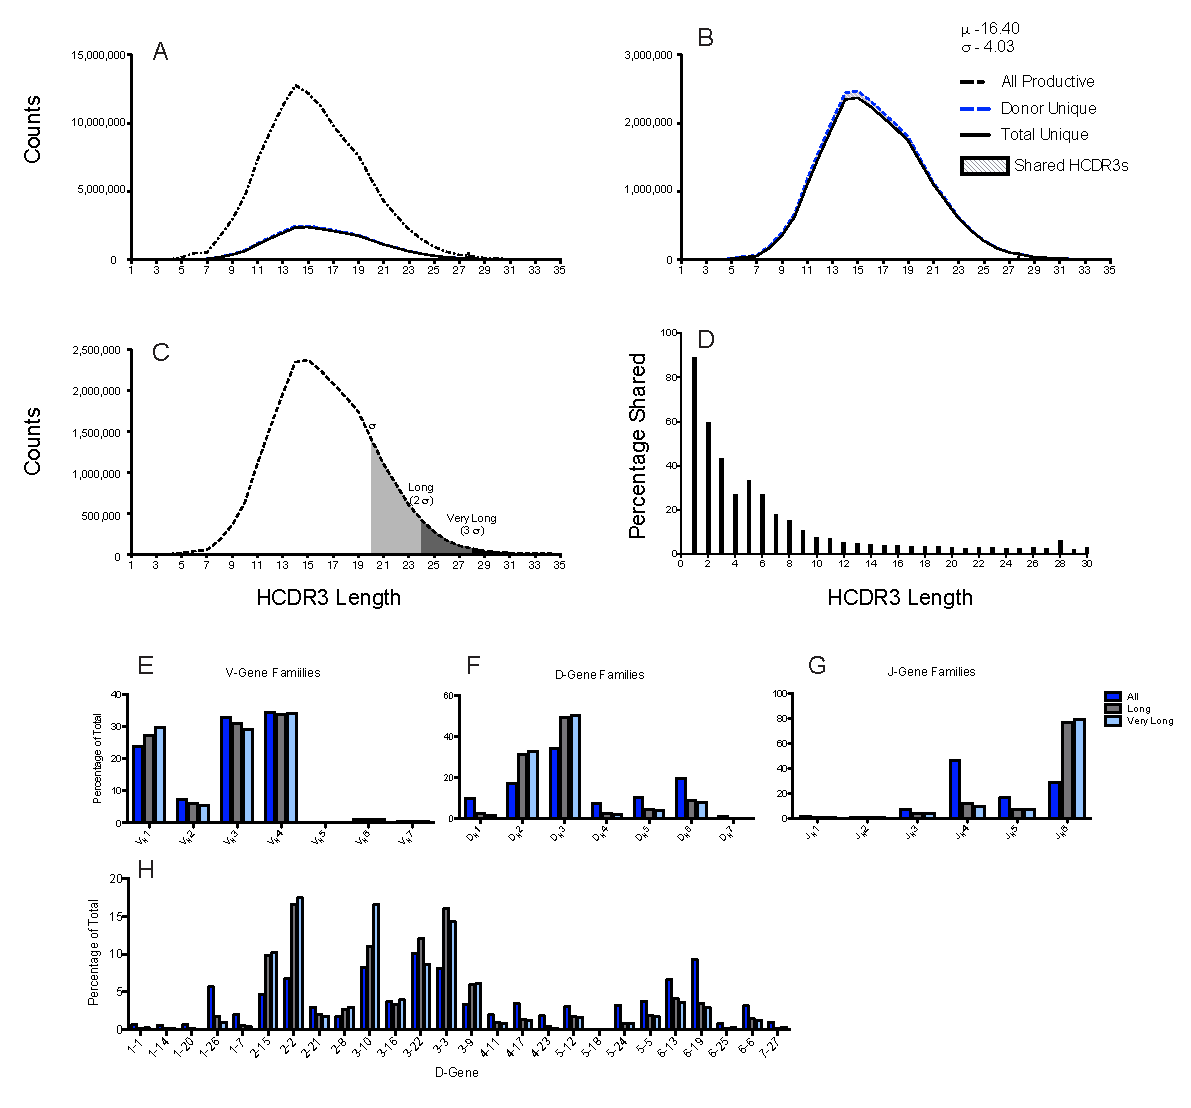
\includegraphics[width=.9\linewidth]{images/chapter3/figure3_7.pdf} % requires the graphicx package
   \caption[Distribution and VDJ gene Usage]{Length distribution for all productive sequences (black dashed line), unique among within each donor (blue dashed) and unique among every donor (black solid) (A). Zoomed in distribution of total unique and donor unique to see overlap. Sequences that are unique between donors are shaded in grey lines (B). Total unique with standard deviations shown at 20, 24, and 28 (C). Percentage of shared sequence as a function of HCDR3 length. Shared sequence is defined as being found in two or more donors (D). V-gene families, D-Gene families and J-Gene family frequencies for all sequences, long, and very long HCDR3 sequences (E, F, G respectively). D-gene families can further be divided into individual gene frequencies for all, long, and very long HCDR3 sequences (H).}
   \label{fig:figure3_7}
\end{figure}
\begin{SCtable}
\centering
\begin{tabular}{rr}
\toprule
\textbf{Metric}        & \textbf{Counts} \\
\midrule
Raw Reads              & 514,312,664     \\
Joined Reads           & 460,931,435     \\
Unique Reads           & 167,667,706     \\
Recombinant Reads      & 159,609,585     \\
Productive CDR3s       & 118,440,255     \\
Unique CDR3s by AA     & 23,357,390      \\
30 Length CDR3s        & 74,457          \\
Unique 30 Length CDR3s & 24,917         \\
\bottomrule
\end{tabular}
\caption[HiSeq 64-Donor Statistics]{Sequencing results from the HiSeq of 64 donors. Raw reads indicate the amount of reads that passed VANTAGE quality metrics. Joined reads are reads that found a paired end partner and could be joined together. Unique reads removed duplicates. Productive HCDR3s are those reads that do not contain a stop codon. Unique CDR3s are those HCDR3s that are not duplicated by amino acid sequence. 30 length HCDR3s are those sequences that are 30 amino acids long by IMGT numbering. Unique HCDR3 sequences are those sequences that are not duplicated in any donor by amino acids.}
\label{tab:table3_2}
\end{SCtable}


\section{Addition of Non-Canonical Amino Acids in Rosetta}
The Rosetta software suite was initially developed for ab initio folding of small globular proteins using fragment-based search methods and knowledge-based potentials to score models46. Because of this, the code for Rosetta made protein amino acid residues the smallest object. All proteins would be made up of residue objects, and all ‘building blocks’ would be made up of parameters that describe your residue object. This made sense at the time of Rosetta’s inception given its primary purpose, but as it’s scoring function was being developed for a wide variety of molecular modeling tasks, the residue based code became difficult to implement for non-residue type molecules, i.e. drug-type ligands, glycans, and post-translational modifications.

The PG9 complex relied on complex and high-mannose type glycans that were bound to asparagine residues at position N160 and N156 (HXBc2 numbering) 19. Removal of these residues abrogated binding to HIV envelope47. Thus, it was necessary to include both of these glycans in our predictions. It was also necessary to encode these glycans as non-canonical amino acid residues rather than post-translational modification due to the residue object requirement of Rosetta score function. We based the protocol of adding the two non-canonical amino acids after the work of Renfrew and colleagues who developed a generalized protocol for implementing non-canonical amino acids into Rosetta48. The protocol used a series of steps that we loosely followed that involved extraction of the residue, minimization of the residue using quantum mechanics simulations, and description of the new amino-acid types as a series of parameters that Rosetta can recognize. We first had to benchmark the non-canonical amino acid types before we could use them in the protocol. To do this we ran minimization and design against the glycan and determined if our best scoring models were the closest to the native structure found in the PDB. The best scoring model according total energy was aligned with the native structure, we saw minimal deviation from the native structure indicating that for good scoring models, the glycan conformation is preserved (figure \ref{fig:figure3_8}A). A general trend between the glycan score and the total score as a function of the glycan RMSD (the deviation from the native conformation) was observed indicating that the glycan tolerating the Rosetta scoring function (figure \ref{fig:figure3_8}B). We also observed that PG9 HCDR3 amino acids were ideal for antibody-antigen complex during redesign of the PG9-antigen (figure \ref{fig:figure3_8}C). With these data, we could proceed with the threading protocol with incorporated glycans.

\begin{figure}
   \centering
   \includegraphics[width=.9\linewidth]{images/chapter3/figure3_8.pdf} % requires the graphicx package
   \caption[Glycan Addition and Benchmarking Template]{Glycan addition and benchmarking template. Energetically minimized loop of the PG9 HCDR3 overlaid on the native PG9-antigen complex (PDB-3U4E).14 Native PG9-antigen is shown in darker colors while the redesigned, energetically minimized and re-docked structures are shown in lighter colors. Light is chain is shown in blue, heavy chain grey, and antigen in magenta. The two glycans are shown in stick representation. The native glycan positions are shown in transparent stick conformation (A). The score of the glycan and the score of the model are shown as a function of the glycan RMSD. On the y-axis are Rosetta scores, and on the x-axis is the glycan RMSD from native structure found in the PDB. The top panel is the total energy of the complex compared with the glycan RMSD while the bottom compares the glycan score to the glycan RMSD. A general trend is shown between the glycan deviation from native conformation and an increase in score (B). Sequence logo of redesigned HCDR3 loop of PG9 with glycans present. The x-axis shows PG9 native sequence (C).}
   \label{fig:figure3_8}
\end{figure}


\section{High-Throughput Threading of HCDR3 Sequences}
We took 4000 random HCDR3 sequences from an available dataset of 26,417 (table \ref{tab:table3_2}). These sequences were “threaded” over the PG9 HCDR3 backbone and energetically minimized. We did not include the antigen in this first set of modeling experiments as it our first goals were to establish a high-throughput prediction model of PG9-like antibodies and not necessarily anti-HIV gp120 neutralizing antibodies. This was for an experimental contingency in case our modeling experiments predicted that none of our sequences could bind gp120 antigen.

The threading protocol removes amino acid sequence identity of the HCDR3 loop and replaces, or “threads”, one of the 4000 random HCDR3 sequences from our dataset. After they amino acid identity has been replaced, the PG9 antibody is energetically minimized and scored with the Rosetta scoring function (detailed in the document introduction).

Considering each model took approximately 1.2 CPU hours to complete at the computing cluster (https://vanderbilt.accre.com) at the time of writing, all 26,417 models would have taken 31,700 CPU hours to complete. Considering Rosetta takes approximately 1000-10000 models to determine energy landscape50-54, we were approaching CPU times from 3.17 x 10$^{7}$–3.17 x 10$^{8}$ hours. I could utilize approximately 600 processors running in parallel, cutting down CPU times to 52,834 hours or ~6 years. Obviously these numbers were unrealistic at the time of writing, so we decided to optimize heuristics methods that could be accomplished with a far fewer number of models. We chose 4000 random sequences with 50 models as a strict cutoff to maximize data output within the capabilities of our computational resources.

To evaluate the threading protocol, we scored our models using the Rosetta scoring function and plotted it against the deviation from PG9s native structure (figure \ref{fig:figure3_9}A). As a control, PG9 and PG16 are also put into the threading protocol to evaluate the scoring functions ability to make distinctions between poor scoring and favorable scoring models. Considering we know that PG9 and PG16 sequences form to PG9s backbone conformation, we expect a very low deviation from PG9s crystal-structure conformation. We also expect Rosetta’s scoring function to score these sequences as favorable relative to many of the random HCDR3s that were evaluated in the protocol. Indeed, we observed that PG9 and PG16 consistently rank as the most favorable in terms of score and conformation and confirm the accuracy precision of our threading protocol (figure \ref{fig:figure3_9}A).

In contrast, the random 4000 HIV-naïve HCDR3 sequences tend to group into three separate categories. Those sequences which maintain the HCDR3 structure of PG9, but score poorly (figure \ref{fig:figure3_9}B), sequences which score well but collapse or deviate away from PG9 native conformation (figure 3.9D), and finally sequences which score well and retain PG9 conformation (figure \ref{fig:figure3_9}C). These three groups give a diverse sequence-energy landscape to be carried on into our heuristics in order to evaluate the remaining ~22,000 HCDR3 sequences.

\begin{figure}
   \centering
   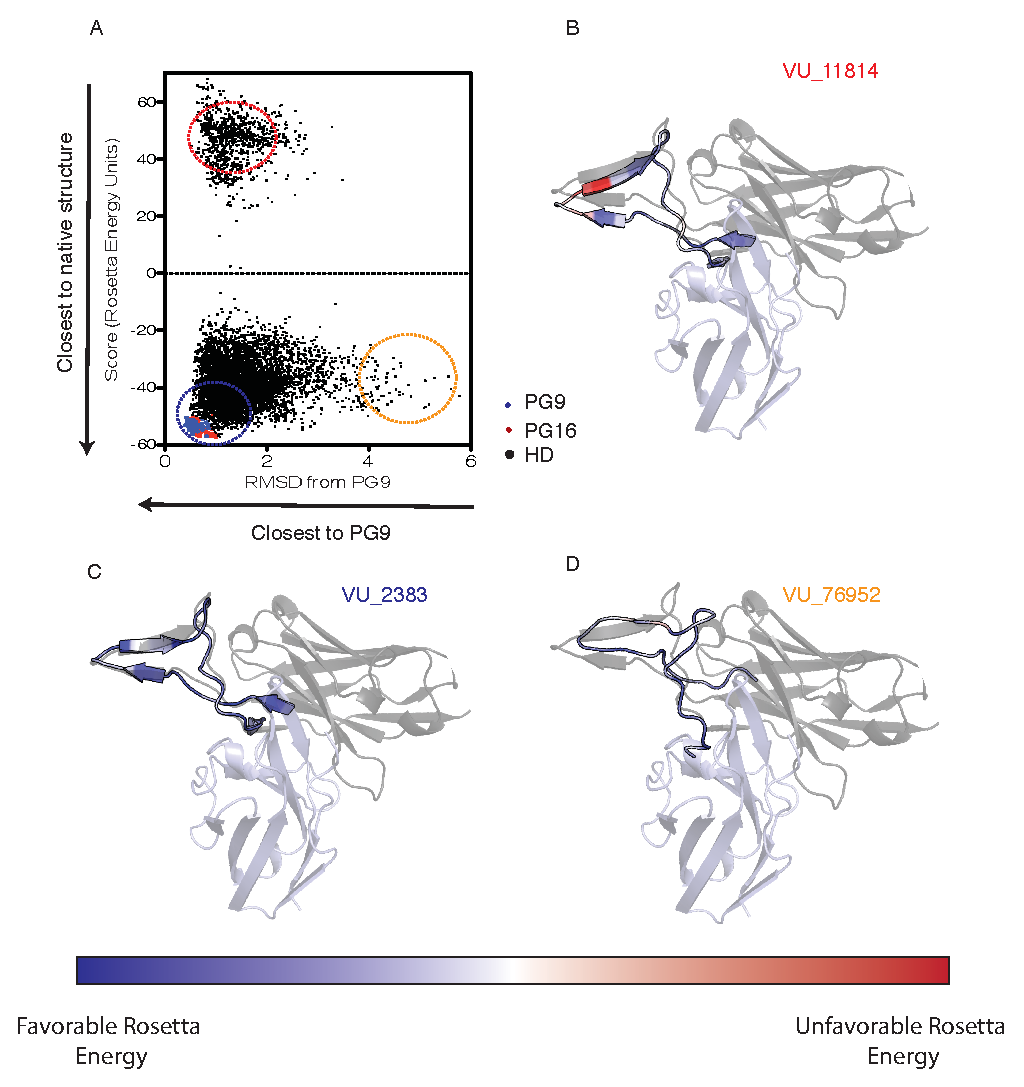
\includegraphics[width=.9\linewidth]{images/chapter3/figure3_9.pdf} % requires the graphicx package
   \caption[Threading PG9 Produces Three Structural Outcomes ]{The threading protocol for PG9 is evaluated for structural mimicry and against the Rosetta scoring function. The models scores are evaluated and plotted against the root mean squared deviation (RMSD) from the native PG9 HCDR3 structure. Lower scoring models are closer to native structure (y-axis) while models closer to PG9 HCDR3 structure have a lower RMSD (x-axis). Repeated measures of PG9 and PG16 are grouped close to native structure and close to PG9 structure (blue and red points) while HIV naïve antibody sequences are shown are labeled HD (black points) (A). For figured B-D, HCDR3 structures are aligned to native PG9 (shown in transparency). The HCDR3s are colored by their Rosetta score with blue being a favorable scoring residue and red being an unfavorable score. There are three different outcomes observed for the threading experiment. Sequences which can retain PG9 structure but produce an unfavorable score (B, dashed red circle in figure A), sequences which produce a favorable score but collapse away from PG9 native structure (D, dashed orange circle in figure A), and sequences which score favorably and adopt PG9 conformation (C, blue dashed circle in figure A).}
   \label{fig:figure3_9}
\end{figure}


\section{Heuristics to Rapidly Score HCDR3 Sequences}
Using the 4000 HIV-naïve HCDR3 sequences, we randomly choose half of the sequences to be in the benchmark set or the training set. For the training set, 2000 sequences were evaluated with the Rosetta scoring function and for each position 96-125 (PDB numbering), we filled a position structure specific scoring matrix (P3SM). For each position, and each amino acid identity, we gave an initial score of 0.0 to baseline yielding a 20 x 30 matrix, and averaged each amino acid identity score at each position (figure \ref{fig:figure3_10}A,B). The matrix can be visualized as a heat map with favorable scores in blue and unfavorable scores in red (figure \ref{fig:figure3_10}B).

The P3SM now becomes our heuristic to rapidly score other sequences that were not run through the computationally expensive threading protocol. We can validate our heuristic by evaluating how well the P3SM does at predicting Rosetta energies by applying it to the other 2000 sequences in the benchmark set. The P3SM may not give absolute Rosetta energies but should provide a relative ranking compared to other HCDR3 sequences. We observe a 0.863 r2-value for a correlation between actual Rosetta energies and P3SM predicted energies. For the top 10\% energies evaluated by the Rosetta energy function, our correlation falls to 0.300 (figure \ref{fig:figure3_10}C).

To determine the relative noise of the P3SM, we ranked the scores and determined the position of PG9. It was found in 104th position out of all 26,417 sequences (0.3\%). The difference in the PG9 P3SM score and the top scoring sequence was 3.82 Rosetta energy units. Thus, the final noise tolerance of our matrix was -34.84 ± 3.82 (-31.02 to 38.66) which encompassed approximately 1000 sequences (figure \ref{fig:figure3_10}D). We then define our P3SM heuristic to be able to accurately pick out the top 1000 out of 26,417 sequences (3.79\%).

\begin{figure}
   \centering
   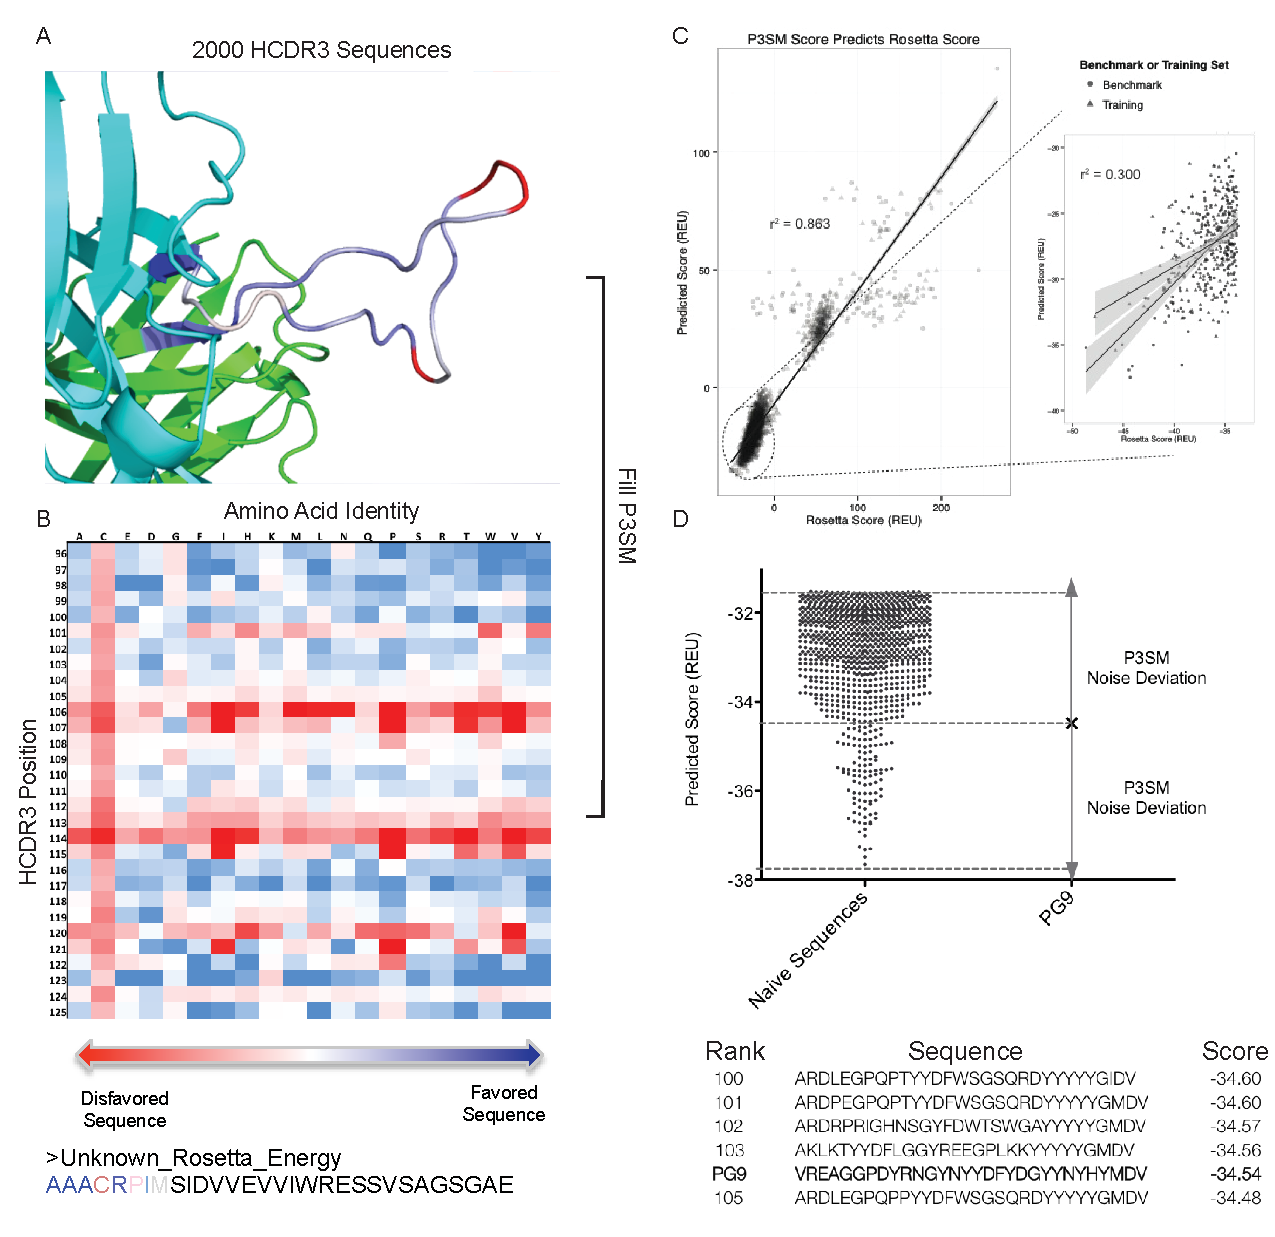
\includegraphics[width=.9\linewidth]{images/chapter3/figure3_10.pdf} % requires the graphicx package
   \caption[Heuristics Predict HCDR3 Sequences that Mimic PG9 Structure]{Heuristics predict HCDR3 Ssquences that mimic PG9 structure. 2000 random models are evaluated at each amino acid position. A cartoon representation of the HCDR3 loop is shown with each position colored with a blue-red gradient according to favorable to unfavorable amino acid identities, respectively (A). Each position is initially assigned a score of 0.0 and enumerated through averaging each amino acid identity with the score to fill a position structure specific scoring matrix (P3SM) from 2000 HCDR3 sequences. The matrix can then be used to rapidly score the other 2000 models that were not used to fill the matrix to predict a Rosetta score (B). A simple linear regression can be applied to the actual Rosetta energy score of a sequence and its predicted score to give a coefficient of determination (r$^{2}$) of 0.863. When only the top 10\% by actual Rosetta score are considered the coefficient of determination drops to 0.330 (C). Using the P3SM, PG9 scored 104th. Calculating the difference in score between the top scoring sequence and PG9 left a noise tolerance of 3.82 Rosetta energy units (REU). Calculating \pm 3.82 REU of PG9 leaves 1000 HCDR3 sequences that fall within the noise tolerance range of the P3SM (D).}
   \label{fig:figure3_10}
\end{figure}


\section{Docking and Minimization of HCDR3 Variants}
With 1000 candidate sequences from the original sequence pool of 26,417, we ran the threading protocol again in the presence of the antigen and complex glycans that were added from earlier sections (see addition of non-canonical amino acids). The threading protocol was modified slightly to include all atom constraints, and an additional docking step and 100 models generated for each sequence (100,000 models). The full protocol is detailed in the methods section of the appendix.
In addition to PG9 deviations and total scores, we also evaluated binding energies, which are the change in free energy (ΔΔG). We define the ΔΔG as follows.

%$\Delta\DeltaG_{Complex} = \deltaG_{Bound} - \deltaG_{Unbound}$

Where,

%$\DeltaG_{Bound} = RosettaScore_{Complex}$ and  $\DeltaG_{Unbound} = RosettaScore_{Seperated}$

We decompose the binding energies, total energies, and deviations into several metrics to evaluate the models. Total energy, binding energy, and deviation (C$\alpha$ - RMSD) for just the HCDR3 portion of the model, the binding energy contribution by both of the glycans (N156 $\delta\delta$G and N160 ΔΔG, HxBC2 numbering), and the total binding energy for the entire model.

Initially each of these metrics can be evaluated individually to see where they rank or in pairs by plotting them against each other (figure \ref{fig:figure3_11}, left panel). Favorable sequences will be in near PG9 in the plot. We can also plot HCDR3 metrics as heat maps and score models qualitatively (figure \ref{fig:figure3_11}, right panel). Both of these methods are inefficient as each metric produces a different rank ordering of the HCDR3 sequences. Therefore, we sought to combine these six metrics into one encompassing score to easily compare where each sequence ranks in comparison to PG9.

To combine the metrics, we assigned a simple Z-score to each metric to find out where that model ranked. The Z-score can then be weighted and averaged for each scoring metric to produce a weighted Z-score that can be used to efficiently rank sequences with one score using the following equation:

$Weighted Z = $

Where w\textsubscript{i} is the weight of each Z-score statistic i, Z\textsubscript{i} is the z score for the statistic i, and N is the total number of statistics. The addition of the weights allowed optimization during ad hoc analysis to ensure PG9 and PG16 were the most favorable weighted Z-score. The final weights used in the protocol were: total ΔΔG – 3.0, HCDR3 ΔΔG - 1.0, HCDR3 total score – 1.0, N156 ΔΔG – 0.5, N160 ΔΔG – 0.5 and HCDR3 C$\alpha$-RMSD - 0.5. We chose the top 80 HCDR3 HIV naïve sequences to carry on to experimental steps, as this number was our upper limit to synthesize.

\begin{figure}
   \centering
   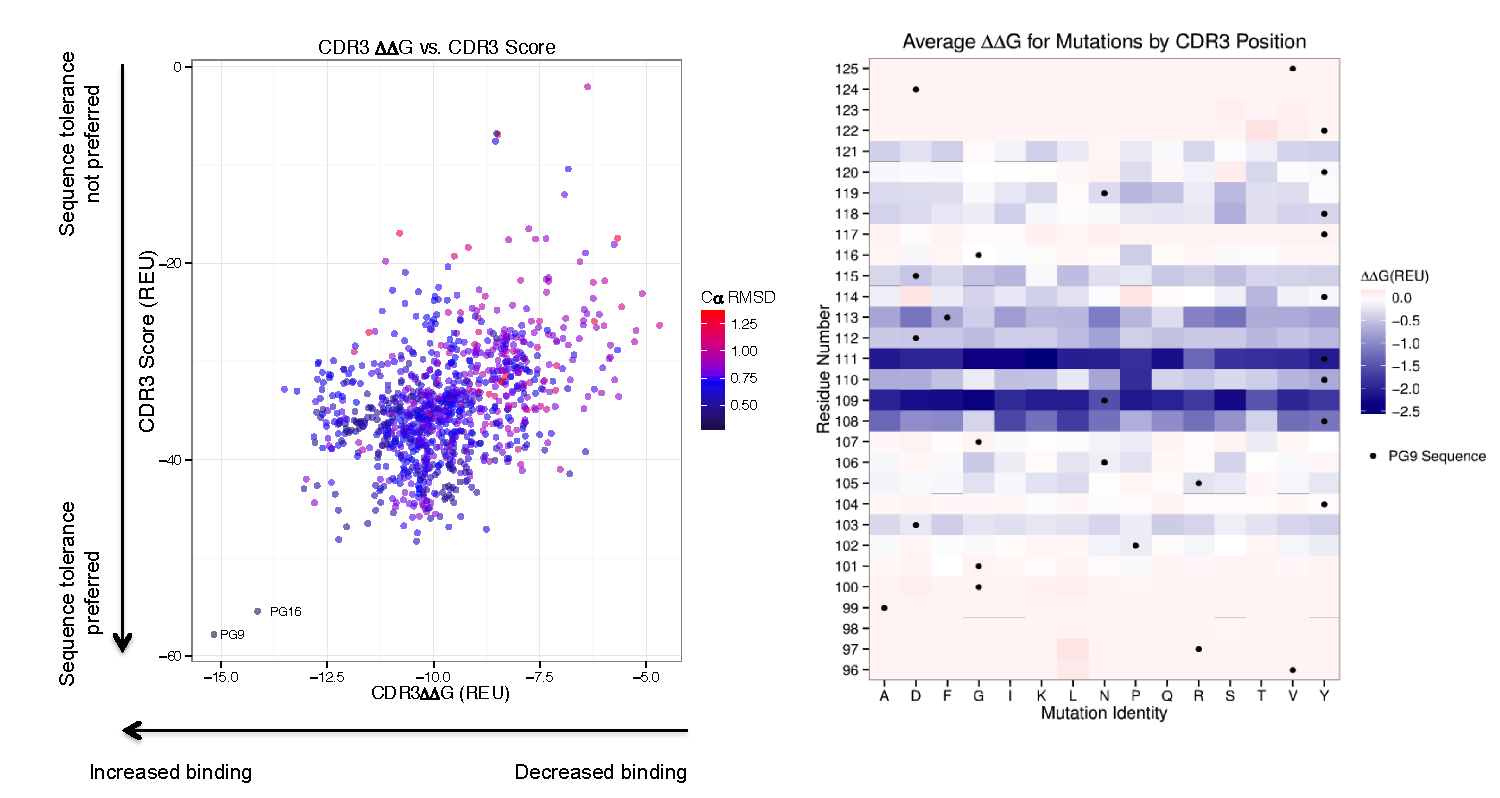
\includegraphics[width=.9\linewidth]{images/chapter3/figure3_11.pdf} % requires the graphicx package
   \caption[Scatter Plots and Heat Maps for P3SM Threading Analysis]{Scatter plots and heat maps for P3SM threading analysis. Each metric can be plotted on a separate axis and sequences which are found to score well are found in the lower left of the graph. For example, HCDR3 binding energy is plotted against HCDR3 score. PG9 and PG16 are found to have favorable binding energy and score (left panel). A heat map can also be generated for each metric for residues in the HCDR3. For example, contribution to binding energy for each amino acid identity can be plotted as a heat map. The red to blue scale is for neutral to favorable reactions (right panel)}
   \label{fig:figure3_11}
\end{figure}

\section{Clustering of HIV-Naïve Sequences}
Rather than synthesize all 80 HIV-naïve sequences that were predicted to be closest to PG9 mimics, we instead considered that several of the sequences were related siblings to each other. Indeed, upon clustering at a threshold 85\% amino acid similarity (4 mutations), the sequences clustered into nine different groups and five sequences formed independent groups (figure \ref{fig:figure3_12}).
We next aligned the nucleotide and amino acid sequences to find sequence similarities among each of our PG9 clustering groups. Surprisingly, only the beginning and end of the sequences corresponding to the base of the HCDR3 displayed a high degree of similarity (figure \ref{fig:figure3_12} A-B).

The similarity arises from the in-frame J\textsubscript{H}-6 gene for most long HCDR3 sequences with the exception of cluster I and IG2, which used J\textsubscript{H}-4 and had significant J-gene exonuclease activity, respectively (table \ref{tab:table3_3}). We also detected some nucleotide conservation for positions 27-36 corresponding to amino acid 9-12, which is a semi-conserved SSGY motif (figure \ref{fig:figure3_12} A-B). Rather than synthesize and express each of the 80 variants, we chose to synthesize one member from each cluster and one of the sequences that did not cluster. These sequences were selected based on their Rosetta weighted Z-score metric within each cluster (table 3.4).

\begin{figure}
   \centering
   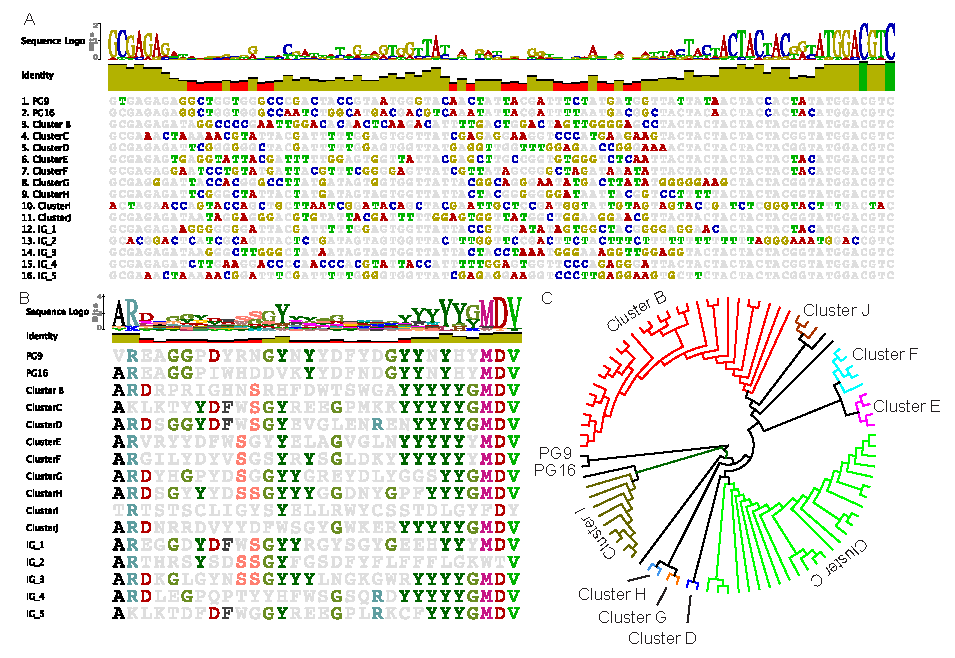
\includegraphics[width=.9\linewidth]{images/chapter3/figure3_12.pdf} % requires the graphicx package
   \caption[PG9-Mimicry Candidates Cluster Into Groups]{PG9-mimicry candidates cluster into groups. The consensus nucleotide sequence is aligned for each cluster B-J. There is little sequence similarity in the junctions except for the VH and JH gene. Sequence logo representations are shown above the sequence to detect conservation. Five independent group sequences are also shown (A). The same as (A) translated. Conserved elements are shown in the JH region due to conserved use of the JH6 gene family (B). The cladogram for each HCDR3 amino acid sequence shows how the top 80 sequences cluster into 9 groups with some groups having multiple sequences that differ by 1-4 amino acid mutations but are derived from the same lineage (C).}
   \label{fig:figure3_12}
\end{figure}
\begin{table}
\centering
\resizebox{.99\linewidth}{!}{
\begin{tabular}{lllllccccc}
\toprule
\textbf{Cluster} & \textbf{Members} & \textbf{V\textsubscript{H}} & \textbf{V\textsubscript{D}} & \textbf{V\textsubscript{J}} & \textbf{V-D Length} & \textbf{D-J Length} & \textbf{D 5'-Exo} & \textbf{D 3'-Exo} & \textbf{J-Exo} \\
\midrule
B                & 29               & V3-07*01    & D3-09*01    & J6*02       & 21                  & 15                  & 3                 & 10                & 2              \\
C                & 25               & V4-34*01    & D3-03*01    & J6*02       & 10                  & 24                  & 0                 & 6                 & 2              \\
D                & 2                & V1-46*01    & D3-03*01    & J6*02       & 9                   & 25                  & 4                 & 6                 & 3              \\
E                & 4                & V1-02*02    & D3-03*01    & J6*03       & 4                   & 23                  & 0                 & 4                 & 0              \\
F                & 5                & V4-34*01    & D3-16*02    & J6*03       & 9                   & 15                  & 4                 & 2                 & 0              \\
G                & 2                & V1-02*02    & D3-22*01    & J6*02       & 16                  & 16                  & 7                 & 3                 & 10             \\
H                & 2                & V4-04*02    & D3-22*01    & J6*02       & 6                   & 23                  & 1                 & 0                 & 8              \\
I                & 9                & V4-34*12    & D2-02*01    & J4*02       & 54                  & 9                   & 4                 & 12                & 2              \\
J                & 3                & V3-07*01    & D3-03*01    & J6*02       & 14                  & 14                  & 0                 & 6                 & 1              \\
IG1              & 1                & V3-07*01    & D3-03*01    & J6*03       & 8                   & 29                  & 2                 & 4                 & 9              \\
IG2              & 1                & V2-70*01    & D3-22*01    & J6*02       & 10                  & 48                  & 3                 & 7                 & 25             \\
IG3              & 1                & V1-02*02    & D3-22*01    & J6*02       & 11                  & 21                  & 6                 & 0                 & 5              \\
IG4              & 1                & V1-03*01    & D3-03*02    & J6*02       & 17                  & 9                   & 0                 & 8                 & 0              \\
IG5              & 1                & V4-34*01    & D3-03*01    & J6*02       & 12                  & 29                  & 2                 & 6                 & 7              \\
PG16             & 1                & V3-33*05    & D3-03*01    & J6*03       & 34                  & 9                   & 1                 & 18                & 2              \\
PG9              & 1                & V3-33*05    & D3-03*01    & J6*03       & 34                  & 0                   & 1                 & 2                 & 9      \\
\bottomrule
\end{tabular}}
\caption[Gene Usage Statistics of PG9-Mimicry Clusters]{Each of the nine clusters and independent sequences (IG1-5) and their representative V, D, and J genes are shown. V-D and D-J lengths are the nucleotide lengths of those junctions. D 5'-, D 3'-, and J-Exo were the amount of nucleotides excised in the junctions to make a productive recombination. Point mutations in the junction are not shown.}
\label{tab:table3_3}
\end{table}



\section{Design of Top PG9-Mimicry Candidates}
We realized that these wild-type sequences sometimes contained clashes or caused other steric strain of the HCDR3 loop that was reflected in the difference in normalized Z-scores (table \ref{tab:table3_4}) or as an energetic gap between the predicted energies of PG9 and the top 80 variants selected (figure \ref{fig:figure3_13}A). It was because of this we decided to run a dock-design protocol that would relieve clashes and strains for unfavorable amino acids. We also imposed a filter that gave bonuses for amino acids that were native to the starting sequence. It was in this way, we were able to attain predicted PG9 mimicry by lowering the energetic gap while retaining as many wild-type sequences as possible (figure \ref{fig:figure3_13})We chose a variant from each cluster whose sequence recovery (the percentage of designed sequences that were wild-type) and carefully analyzed each predicted mutation suggested by Rosetta. We ranked the mutations based on a fitness score. We defined the fitness core as the change in total score for the mutation from the wildtype added to the change in binding energy for the mutation compared to wildtype. If the fitness was found to be significant, the mutation was confirmed by visual inspection.

Briefly, I will explain the rationale for choosing the mutations for cluster B. Variant VU42252 was chosen as the representative candidate for design since it provided the best sequence recovery to the wild-type sequence as well as beneficial fitness (figure \ref{fig:figure3_14}A). Each mutation is plotted as a function of its fitness and grouped together by position (figure \ref{fig:figure3_14}B). If there is a large decrease in energy from the wild-type sequence, it corresponds to a beneficial fitness for a given mutation. Those mutations that had a favorable change in fitness with a magnitude of greater than 1.5 Rosetta energy units were manually inspected (figure \ref{fig:figure3_14}C,D). Two such mutations are shown at position 106 (figure \ref{fig:figure3_14}C) and position 120 (figure \ref{fig:figure3_14}D). For position 106, the wildtype serine is not preferred since it leaves a large exposed gap between the antigen face and the antibody interface. Upon mutation to an asparagine, the gap is filled in. Additionally the asparagine makes new hydrogen bond contacts with the antigen. This is predicted to benefit the binding energy and stabilization of the complex. Position 120 has a wild-type tyrosine that repels against the large steric bulk of the glycan. A mutated asparagine at this position allows an inter-HCDR3 hydrogen bonds to stabilize the loop while also making additional hydrogen bonds to the glycan.

For cluster B, we chose six different positions to be mutated alone or in combinations that produced five different candidate variants. This totals six different variants to try for cluster B, one wildtype sequence, and five mutational variants that range from 3-10 mutations. The remaining clusters were analyzed similarly and in total, 10 wildtype sequences were chosen for experimental characterization and 74 different sequences that were mutational variants of the representative cluster sequence.

\begin{table}[!h]
\centering
\begin{tabular}{lc}
\textbf{Cluster}   & \textbf{Weighted Z-Score} \\
\hline
Cluster B & -1.24            \\
Cluster C & 0.28             \\
Cluster D & 0.11             \\
Cluster E & 0.15             \\
Cluster F & -0.34            \\
Cluster F & -0.20            \\
Cluster G & 0.31             \\
Cluster H & 0.11             \\
Cluster I & -2.54            \\
Cluster J & 1.48             \\
PG9       & -4.80            \\
PG16      & -1.87            \\
IG 4      & -1.46
\end{tabular}
\caption[Weighted Scores of PG9-Mimic Clusters]{Weighted scores of PG9-mimic clusters. The top scoring sequence for each cluster are shown with weighted the Z-score.}
\label{tab:table3_4}
\end{table}
\begin{figure}
   \centering
   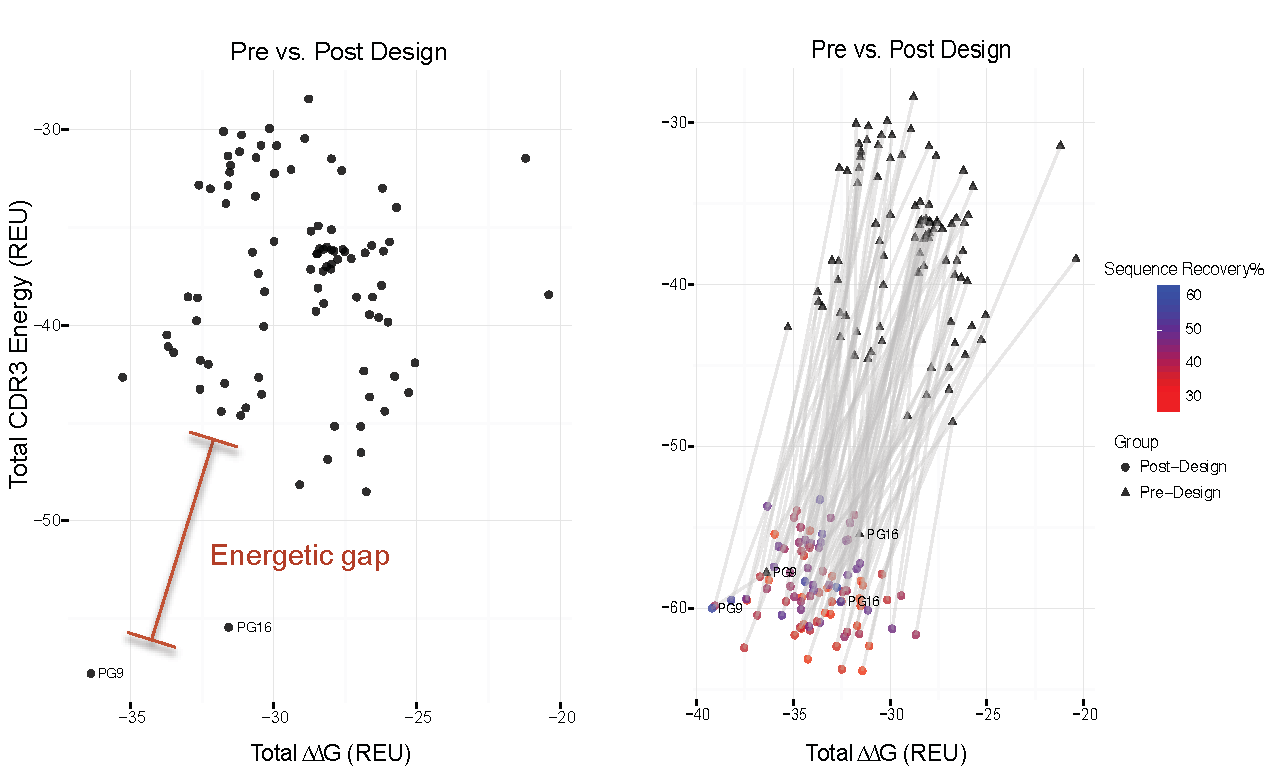
\includegraphics[width=.9\linewidth]{images/chapter3/figure3_13.pdf} % requires the graphicx package
   \caption[Energetic Barriers for Complete PG9-Mimicry]{Energetic barriers for complete PG9-mimicry. The total HCDR3 energy and binding energy are plotted for the top 80 sequences selected by normalized Z-score as well as PG9 and PG16. There is a significant energetic gap between these sequences and complete PG9 mimicry (A). After redesign, the sequences approach the energy of PG9 and PG16 (shown as connecting triangles to circles). The blue-red scale is the sequence recovery percentage indicating how much of the wild-type sequence is retained.}
   \label{fig:figure3_13}
\end{figure}
\begin{figure}
   \centering
   \includegraphics[width=.9\linewidth]{images/chapter3/figure3_14.pdf} % requires the graphicx package
   \caption[Mutation Analysis of Cluster B]{Mutation analysis of cluster B. A sequence logo representation of the cluster B variant with the best sequence recovery is shown. The wild-type sequence of the cluster B candidate named VU42252 is plotted on the x-axis. The preferred mutations for each position in the HCDR3 are shown on the y-axis with the height of each letter corresponding to Rosetta’s preference for that mutation (A). Each mutation that was predicted to benefit fitness is plotted by position. The more preferred mutations correspond to a more negative number. A cutoff threshold of 1.5 Rosetta energy units is shown as a dashed line to indicate mutations that were considered for experimental characterization after manual inspection (B). Manual inspection of the mutation at position 106 from the wildtype serine (left panel) to asparagine (right panel). The antigen is shown in beige or gray, for the wildtype and mutation, respectively. The surrounding residues are colored in yellow. The HCDR3 loop is colored blue. The asparagine hydrogen bonds to the antigen, which favors binding energy and stabilization of the HCDR3 loop (C). Manual inspection of position 120 is plotted with the HCDR3 loop in light blue, the heavy chain in green, and the light chain in cyan. The glycans are shown in stick representation. The designed asparagine compared to the wild-type tyrosine makes inter-HCDR3 stabilizing hydrogen bonds as well as additional bonds with the glycan (C).}
   \label{fig:figure3_14}
\end{figure}

\section{Synthesis and Screening of PG9-Mimics}
For the 84 variants, we chose a synthesis strategy that would allow us to swap in HCDR3 sequences with unique cloning sites rather than resynthesize the framework and HCDR1-2 sequences redundantly. It was to this end that I put in a BsiWI at the 5’ end and an XhoI site at the 3’ end of the HCDR3 sequence. Using these cloning sites, small gene fragments could be synthesized rapidly and cost-effectively.
We fully expected not all of the 84 variants to express or bind HIV gp120 and decided to screen each candidate for binding and expression on a small scale.  We made 30 mL test cultures to screen the supernatants for the presence of IgG antibody and its ability to bind gp120 protein.

According to the literature cited by McLellan et al., only certain gp120 monomers bind to PG9 using enzyme-linked immunosorbent assays (ELISA) while PG16 binds gp120 monomers very weakly. Therefore, we combined fifteen different gp120 variants into an antigen cocktail to maximize the chances of binding to each of our 84 PG9-mimics. This cross screening for antibody expression and antigen binding would pre-emptively select which of our 84 candidates should be carried on to upscale expression.
Figure 3.14 plots our screening metrics for expression and binding. We binned each candidate to either be further be characterized, or not further characterized. We based this on an expression cutoff of at least 300 μg/L and a binding of at least 1 OD at maximal concentration.  For some antibodies that did not express well but showed some binding activity, we chose to carry on to further experimentation. The results are summed in Table 3.5 with 35 variants to be expressed at a larger scale. For these, we choose either a 300 mL expression (10 fold) or a 1L expression based on initial expression levels. These antibodies were purified and carried on to biophysical characterization and neutralization studies. With the exception of cluster I, there was at least one candidate from every cluster that would be further characterized (Table 3.5).

\section{Biophysical Characterization of PG9-Mimics}
We chose to use 8 gp120 monomers based on the ability of PG9 to bind them using our ELISA experimental conditions. These monomers contained 5 clade B variants (BaL.01, SC422661.8, 6535.3, RHPA4259.7, and TRJO4551.58), 2 clade C variants (CAP45.2.00.G3, ZM109F.PB) and 1 laboratory adapted SHIV chimera (HXBc2P3.2). We found that PG9 bound these 8 candidate monomers based on previous literature1 and our own pilot studies (chapter IV). We coated each plate in a 384-well format with gp120 monomer and tested binding to the purified 35 variants we analyzed based on our expression/binding sieve analysis in the previous section. Due to replication of these experiments, and consequently the amount of protein used, 4 variants were lost leaving a total of 31 variants analyzed. We calculated effective concentration at half-maximal binding (EC50) of each variant against 8 gp120 monomers. We started our dilution at a very high concentration in order to detect weakly binding antibodies. We set our cutoff for binding at EC50 less than 100 μg/mL.
Not surprisingly, most variants did not bind with the same breadth and potency of PG9. In fact, 16 of the variants characterized did not reach our threshold of binding for any of the monomers tested (figure 3.15, 3-16). However, we found at least one gp120 monomer that bound fifteen of our variants with an EC50 less than 100 μg/mL. We find the easiest monomers to bind are BaL.01, ZM109F.PB, and CAP45.2.00.G3. Our broadest antibody is VU43171_6MUT from cluster C, which bound 7 out of 8 gp120   monomers (figure 3.15, 3-16). Our most potent antibody is VU28693_5MUT from cluster E, which binds ZM109 and BaL.01 with a potency of 1 μg/mL. For comparison, PG9 binds ZM109 and BaL.01 with an EC50 of 0.03 μg/mL and 0.06 μg/mL, respectively. We also had a complete wild-type antibody, that is, an antibody with no design modifications from Rosetta bind BaL.01 and ZM109 at 3.7 μg/mL and 3.6 μg/mL, respectively.

\section{Neutralization of HIV by HIV-Naïve PG9-Mimics}
From the literature, we know that changes in the HCDR3 loop sequence can dramatically alter specificity17,18,20. For instance, making a PG9 HCDR3 with a PG16 backbone was able to neutralize additional viruses, while PG16 HCDR3 with PG9 backbone was also able to pick up additional breadth18.
The exact molecular mechanisms that allow PG9 to bind most gp120 monomers and PG16 weakly bind gp120 monomers is currently unknown1. Both PG9 and PG16 also do not bind gp120 monomers there are able to neutralize indicating their preference for a trimer specific conformation. It was because of this, we decided to test 31 out of our 35 HCDR3 variants for neutralization against pseudoviruses which present native trimer55. We decided to send our variants to a collaborator, Dr. David Montefiori who initially worked out multiple neutralization assays to test recombinant HIV variants56.
It would stand to reason that the relatively large EC50 returned in the binding studies would generate equally large IC50 from the neutralization assays. It was because of this, that we decided to start the concentrations at 100 μg/mL for the neutralization screen. This made our neutralization screen protein-limited and at the time of publication, we could only test two viruses, RHPA and RHPA.N160A. From Figure 3.16, it is evident that this virus is difficult to neutralize and are currently pursuing studies of much weaker viral strains derived from the literature and Figure 3.17. Regardless, VU30400_7MUT from group G was able to neutralize RHPA at 49.3 μg/mL while PG9 neutralized at 6.22 μg/mL. Both of mAbs lost the ability to neutralize RHPA.N160A, a knockout mutation for this class of antibody which removes the large glycan at position 160 indicating its mimicry of PG947.

\section{Analysis of Mutations with Rosetta}
Lastly, we wanted to analyze the binding antibodies for sequence conservation to see if there were any trends. Indeed, figure 3.17 shows antibodies that bound BaL.01 with an EC50 less than 55 μg/mL. The neck of the HCDR3 loop showed great sequence conservation for residues 95-97 with a VRE or VRD, and residues 118-125 with a YYYYMDV, the wild type sequence of an unmutated JH6 gene. These trends were observed for long HCDR3 class of antibodies in recent clustering studies57. I was more interested in conserved sequence elements that would be at the antigen interface. For those residues, there was great sequence divergence and only a few conserved elements were observed. An aromatic residue at position 104, an asparagine, glycine, and tyrosine and for positions 106-108. These sequences fall at a critical hairpin loop that is necessary to make the crucial turn in order to align the beta-sheets necessary for making contact with the antigen. Indeed, Rosetta preferred very few residues at this position due to the non-canonical torsions that were adopted. Other than those sequence elements, we see great sequence diversity, particularly in the contact residues predicted from the crystal structure and homology models (figure 3.17).

\section{Conclusions and Future Directions}
A protective vaccine against HIV-1 will likely involve an elicitation of a broadly neutralizing serum58-63. There are a limited number of neutralizing targets for these bNAbs and include the CD4-binding site, the V3-loop, the V1/V20-loop, membrane proximal region (MPER), and the outer N332 glycans64. Here, we aim to target the V1/V2 loop due to the ubiquity of patients infected with HIV to target this region with neutralizing antibodies64-67. As discussed in the introduction, the RV144 trial, the only HIV vaccine trial to date to show modest efficacy, showed that the correlates of protection were the elicitation of V1/V2 binding mAbs and selective pressure on the V2 region of HIV env44,68.
Recently, a long HCDR3 V1/V2 binding pathway has been elucidated for potent bNabs16. A patient from the CAPRISA cohort developed HIV and they found a modestly potent neutralizing antibody at week 58 post-infection with an HCDR3 length of 35 amino acids. In parallel they had also been taking PBMC samples at various time points throughout infection to find the pathway for the development of these neutralizing antibodies. Using pyrosequencing, they find an unmutated antibody at week 30-38 with no VH or VK gene mutations. Longitudinal sequencing analysis shows this antibody mutating away from the unmutated common ancestor (UCA) and pick up potency with a total of 14 mutations in the HCDR3 regions (40\% mutation) at 58 weeks but relatively few mutations away from the germline sequence (16\%). They showed up to 54\% mutations from the UCA in the HCDR3 with a neutralization breadth up to 47\%. This study shows the tremendous range of sequence diversity that can converge onto one epitope while maximizing breadth and potency. This study is exceptional in its design but does leave some unanswered questions. Firstly, they only derive their antibodies from VH3-30 sequences. This leaves out a tremendous amount of potential recombinations that could become neutralizers. It also focuses on one UCA phylogeny and patient. Although the UCA is said to be available at the original time of recombination, there is no evidence that it is in completely HIV naïve individuals as it was detected at 30-38 weeks post-infection. This is not a true HIV-naïve study as it attempts to characterize the developmental pathways of V1/V2 binders post-infection.
Our study is potentially superior as we interrogate the long HCDR3 repertoire prior to infection. We use 64 different donors maximizing our sequence pool and diversity. We also use a deeper sequencing method to get the depth necessary to characterize such a broad repertoire. Our addition of computational design and bioinformatically driven heuristics instead of brute-force characterization allows us to interrogate the tremendous sequence diversity of the HIV-naïve repertoire. We aimed to answer a simple question. Do HIV-naïve donors possess long HCDR3 sequences that potentially bind and neutralize HIV? If not, will minimal mutations allow them to bind and neutralize V1/V2 epitopes?
The approach to answering these questions involves a four-part strategy that marries computational and experimental methods in order to investigate the HIV-naïve repertoire. First, we used deep sequencing to accumulate a vast pool of HCDR3 sequences. We then used bioinformatics analysis with new algorithms to determine 30-length HCDR3 sequences. Using Rosetta, we used these sequences to establish a heuristic that would let us rapidly evaluate 30 length HCDR3 sequences for their ability to form a PG9-type loop. This allowed us to trim down our vast sequence pool to a manageable amount of HCDR3 sequences to determine experimentally. RosettaDesign allowed us to simulate the process of somatic mutation by applying minimal designs to our sequences in order to enhance potency and breadth.
We experimentally characterized 84 variants, a combination of 10 clusters returned from the computational predictions and 74 combinations of mutations predicted to enhance binding. Of those, we trimmed the number down to 31 due to a lack of expression or initial binding. Of the 31 antibodies, we performed ELISA experiments on 8 representative monomers finding that a total of thirteen including two wild-type sequences have an EC50 less than 50 μg/mL, well within our tolerance to be considered a binder. For our neutralization work, one antibody neutralized a tier-2 virus with a 7-fold lower potency than PG9. We expect that many more of our variants will neutralize given the right experimental conditions. The tier-2 virus is ambitious and we expect that a tier-1 virus, or the env sequences that our variants were designed against, may be potentially easier to neutralize.
Our work has several implications for vaccine design as it demonstrates that multiple HIV-naïve donors contain long HCD3s with the ability to bind gp120. This demonstrates how close an HIV-naïve donor is to actually eliciting a mAb that mimics a broad and potent V1/V2 binder. It was long thought that a repeated vaccination schedule that would gradually induce the necessary somatic mutations to recapitulate the broad and potent antibodies that bind the CD4-binding site. Here we show that an average HIV-naïve donor is closer to producing a broadly neutralizing mAb than initially hypothesized15. This potential paradigm shift in vaccine design would aim to prime for these B-cells with long HCDR3s and then boost for specificity offering protection from HIV-1 challenge.


% % \begin{figure}
% %    \centering
% %    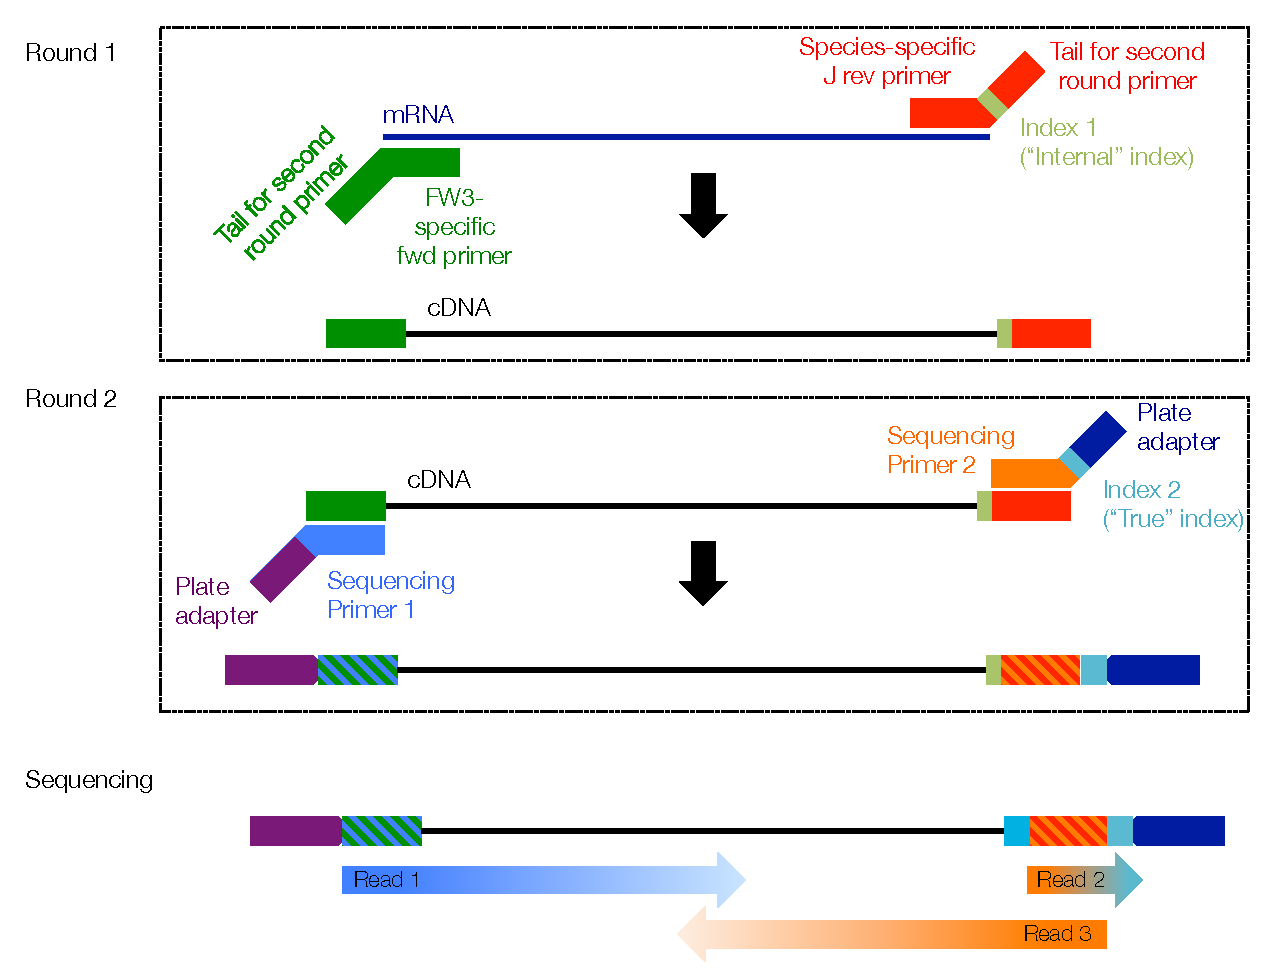
\includegraphics[width=.9\linewidth]{images/chapter3/figure3_6.pdf} % requires the graphicx package
% %    \caption[Current Sequencing Technologies]{Current sequencing technologies. On the x-axis is the current read length for each sequencing platform. The y-axis is the bases per run. Each point is a new iteration of that platforms sequencing read length and coverage. HiSeq has the most coverage with relatively short read lengths. Figure adapted from \citep{developmentinNGS:2012bs} }
% %    \label{fig:figure3_6}
% % \end{figure}

% % \begin{figure}
% %    \centering
% %    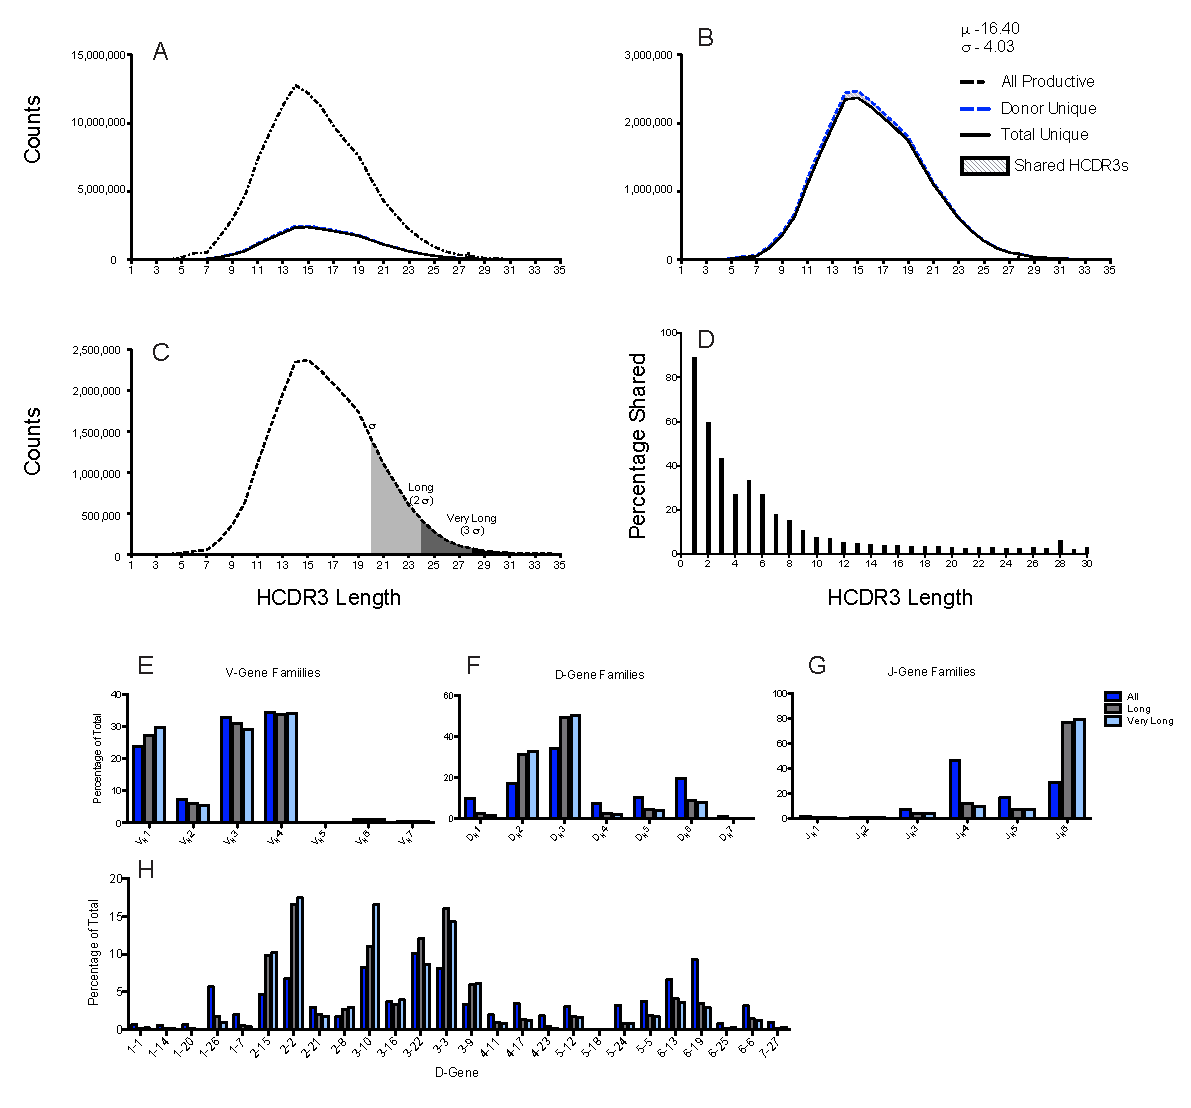
\includegraphics[width=.9\linewidth]{images/chapter3/figure3_7.pdf} % requires the graphicx package
% %    \caption[Current Sequencing Technologies]{Current sequencing technologies. On the x-axis is the current read length for each sequencing platform. The y-axis is the bases per run. Each point is a new iteration of that platforms sequencing read length and coverage. HiSeq has the most coverage with relatively short read lengths. Figure adapted from \citep{developmentinNGS:2012bs} }
% %    \label{fig:figure3_7}
% % \end{figure}

% % \begin{figure}
% %    \centering
% %    \includegraphics[width=.9\linewidth]{images/chapter3/figure3_8.pdf} % requires the graphicx package
% %    \caption[Current Sequencing Technologies]{Current sequencing technologies. On the x-axis is the current read length for each sequencing platform. The y-axis is the bases per run. Each point is a new iteration of that platforms sequencing read length and coverage. HiSeq has the most coverage with relatively short read lengths. Figure adapted from \citep{developmentinNGS:2012bs} }
% %    \label{fig:figure3_8}
% % \end{figure}

% % \begin{figure}
% %    \centering
% %    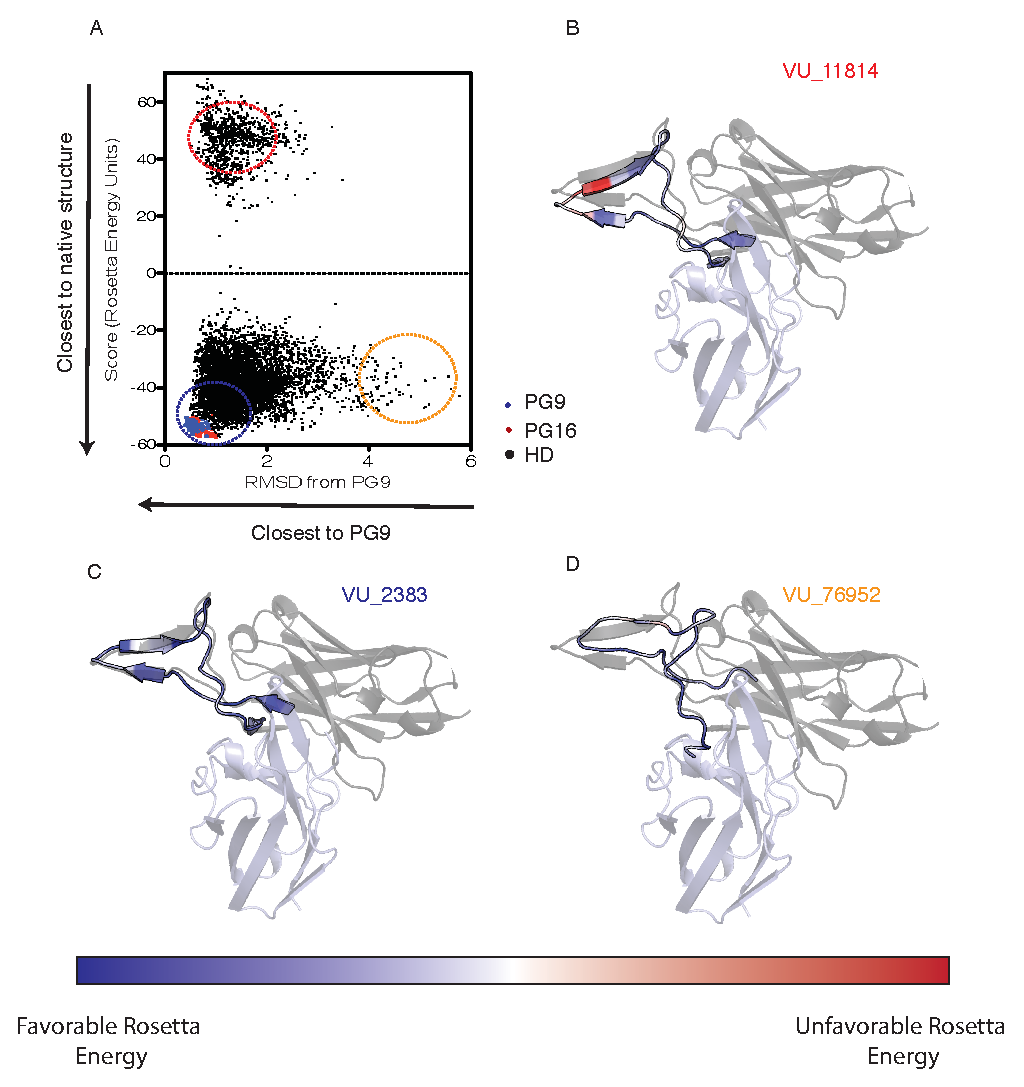
\includegraphics[width=.9\linewidth]{images/chapter3/figure3_9.pdf} % requires the graphicx package
% %    \caption[Current Sequencing Technologies]{Current sequencing technologies. On the x-axis is the current read length for each sequencing platform. The y-axis is the bases per run. Each point is a new iteration of that platforms sequencing read length and coverage. HiSeq has the most coverage with relatively short read lengths. Figure adapted from \citep{developmentinNGS:2012bs} }
% %    \label{fig:figure3_9}
% % \end{figure}

% % \begin{figure}
% %    \centering
% %    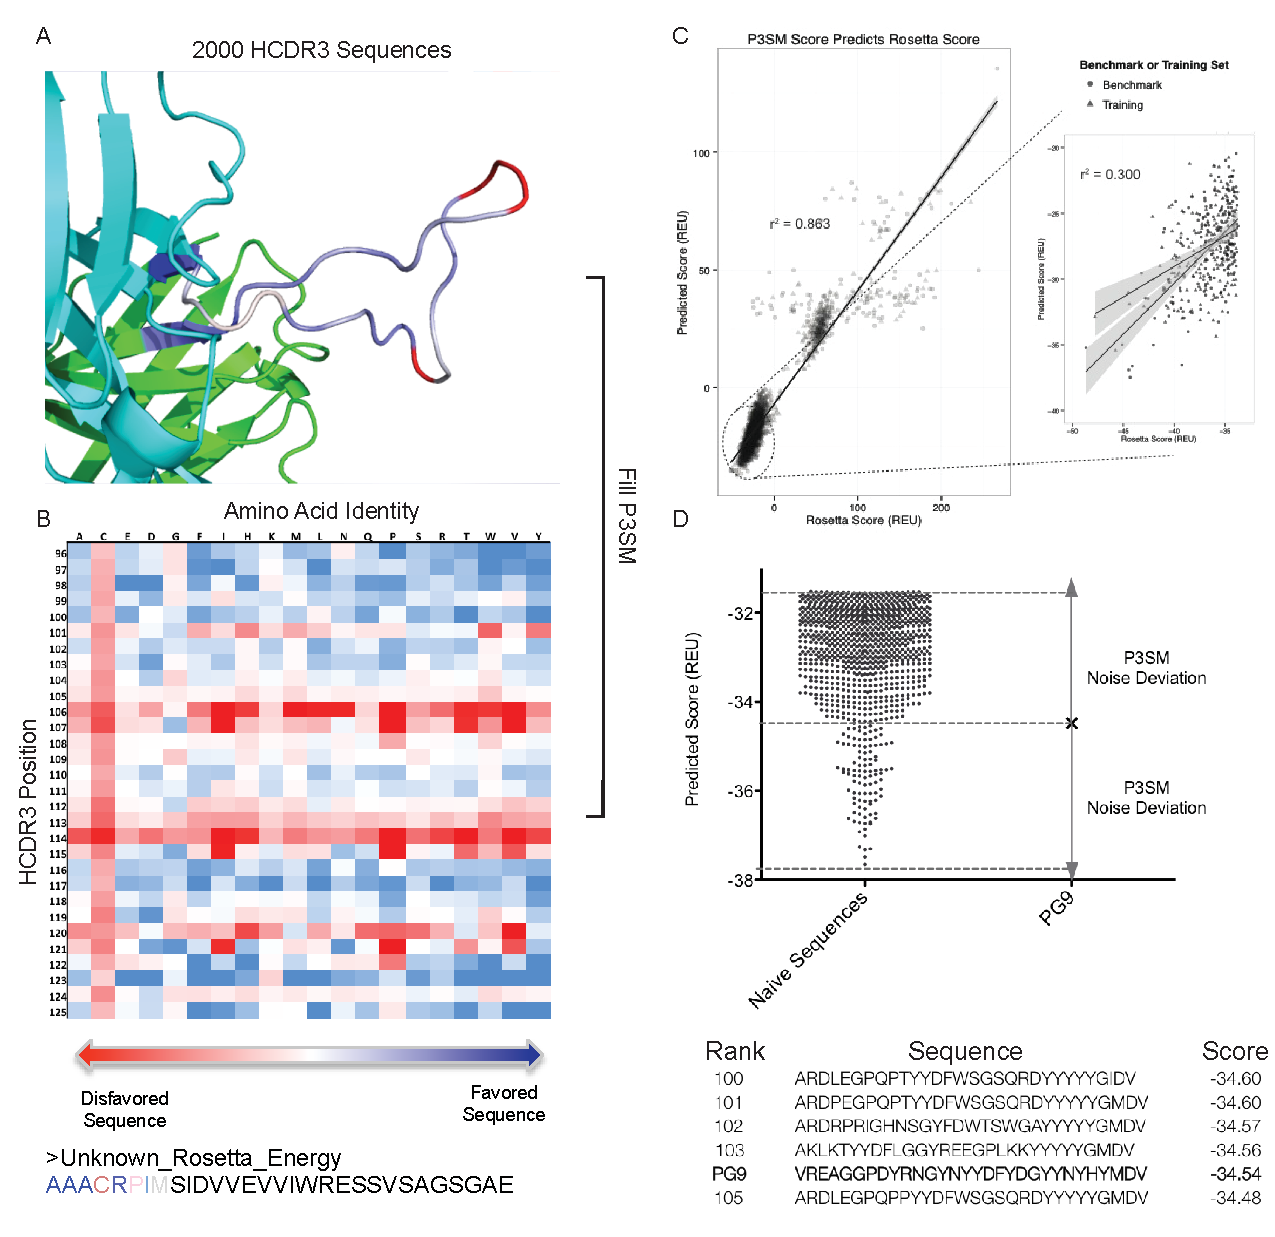
\includegraphics[width=.9\linewidth]{images/chapter3/figure3_10.pdf} % requires the graphicx package
% %    \caption[Current Sequencing Technologies]{Current sequencing technologies. On the x-axis is the current read length for each sequencing platform. The y-axis is the bases per run. Each point is a new iteration of that platforms sequencing read length and coverage. HiSeq has the most coverage with relatively short read lengths. Figure adapted from \citep{developmentinNGS:2012bs} }
% %    \label{fig:figure3_10}
% % \end{figure}

% % \begin{figure}
% %    \centering
% %    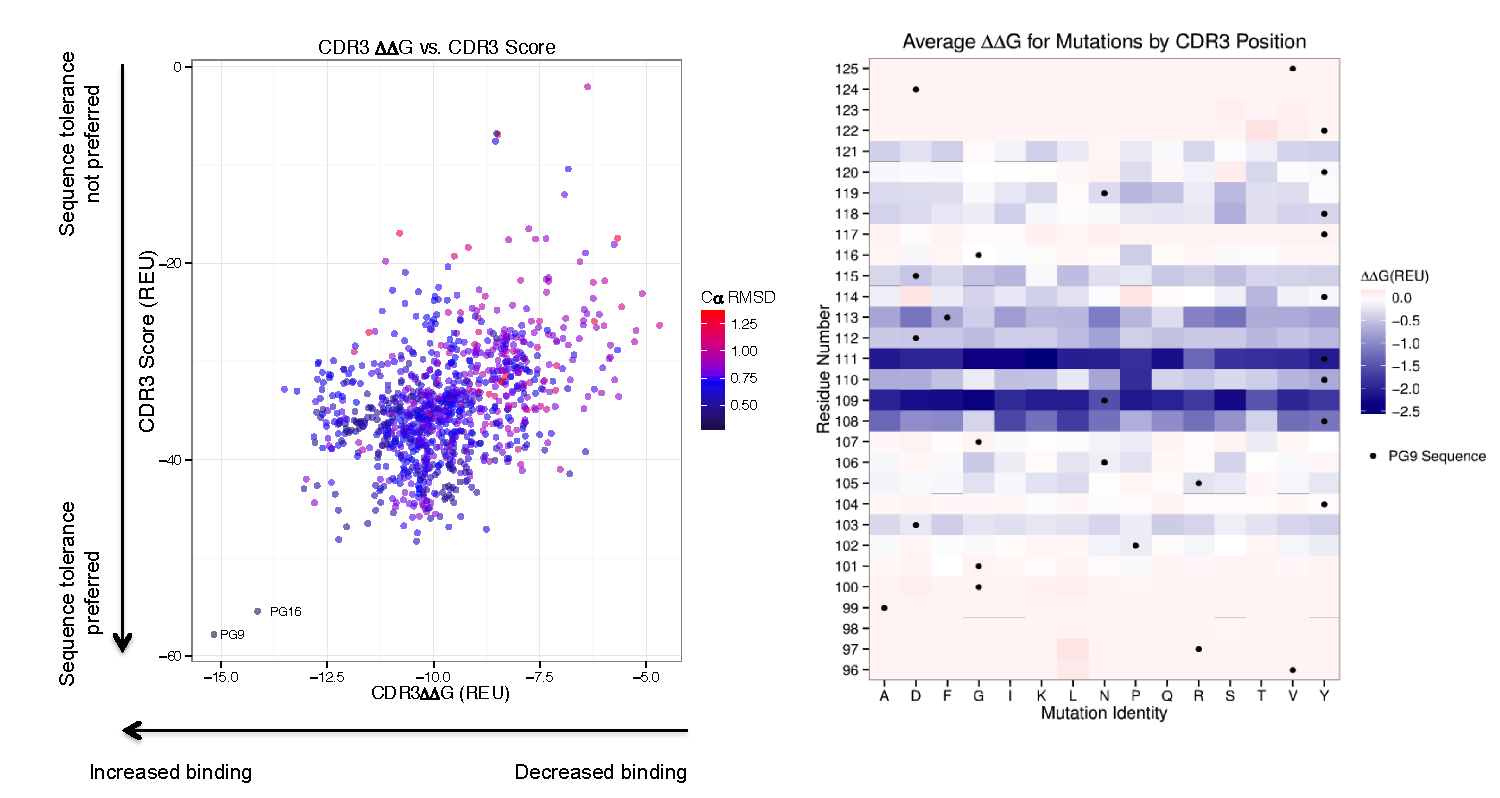
\includegraphics[width=.9\linewidth]{images/chapter3/figure3_11.pdf} % requires the graphicx package
% %    \caption[Current Sequencing Technologies]{Current sequencing technologies. On the x-axis is the current read length for each sequencing platform. The y-axis is the bases per run. Each point is a new iteration of that platforms sequencing read length and coverage. HiSeq has the most coverage with relatively short read lengths. Figure adapted from \citep{developmentinNGS:2012bs} }
% %    \label{fig:figure3_11}
% % \end{figure}

% % \begin{figure}
% %    \centering
% %    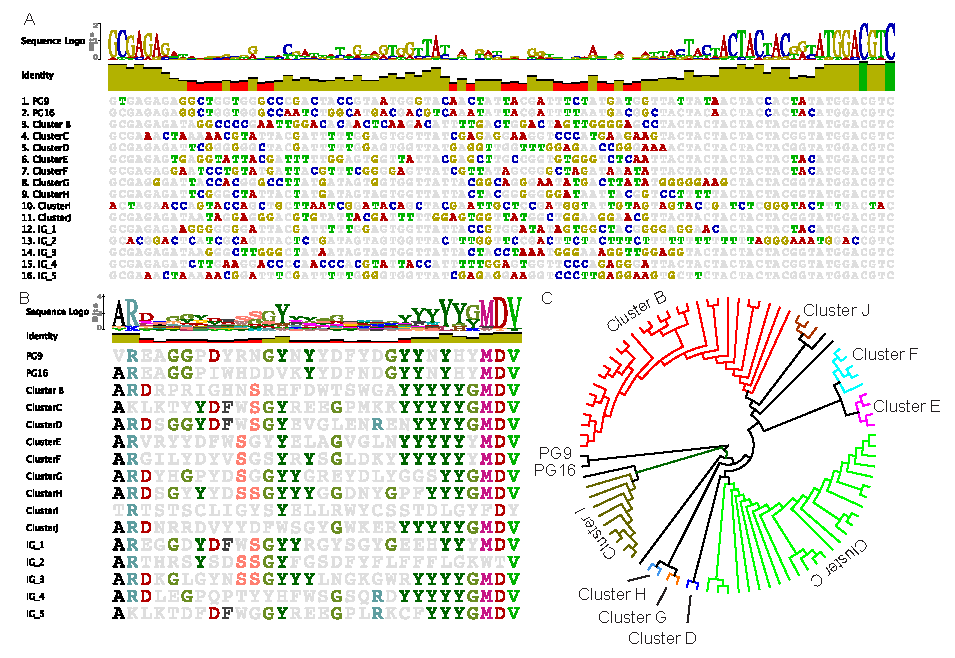
\includegraphics[width=.9\linewidth]{images/chapter3/figure3_12.pdf} % requires the graphicx package
% %    \caption[Current Sequencing Technologies]{Current sequencing technologies. On the x-axis is the current read length for each sequencing platform. The y-axis is the bases per run. Each point is a new iteration of that platforms sequencing read length and coverage. HiSeq has the most coverage with relatively short read lengths. Figure adapted from \citep{developmentinNGS:2012bs} }
% %    \label{fig:figure3_12}
% % \end{figure}

% % \begin{figure}
% %    \centering
% %    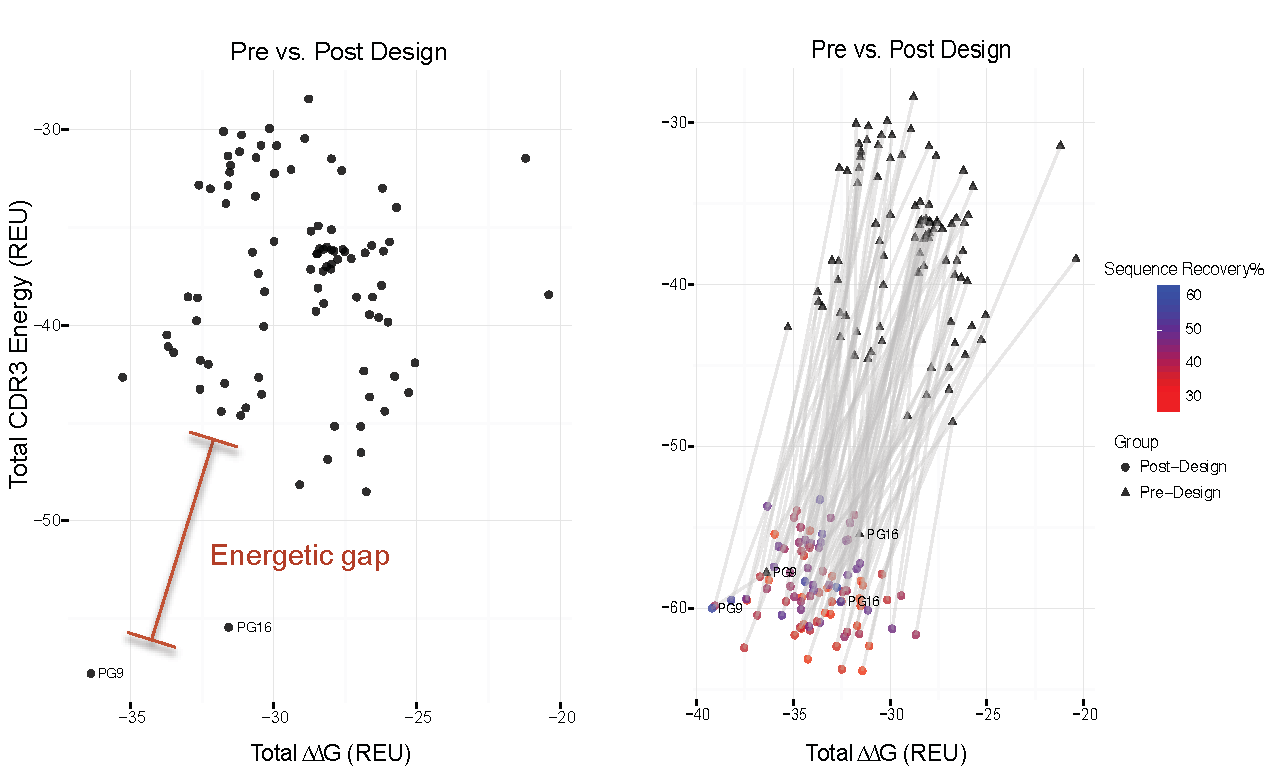
\includegraphics[width=.9\linewidth]{images/chapter3/figure3_13.pdf} % requires the graphicx package
% %    \caption[Current Sequencing Technologies]{Current sequencing technologies. On the x-axis is the current read length for each sequencing platform. The y-axis is the bases per run. Each point is a new iteration of that platforms sequencing read length and coverage. HiSeq has the most coverage with relatively short read lengths. Figure adapted from \citep{developmentinNGS:2012bs} }
% %    \label{fig:figure3_13}
% % \end{figure}

% % \begin{figure}
% %    \centering
% %    \includegraphics[width=.9\linewidth]{images/chapter3/figure3_14.pdf} % requires the graphicx package
% %    \caption[Current Sequencing Technologies]{Current sequencing technologies. On the x-axis is the current read length for each sequencing platform. The y-axis is the bases per run. Each point is a new iteration of that platforms sequencing read length and coverage. HiSeq has the most coverage with relatively short read lengths. Figure adapted from \citep{developmentinNGS:2012bs} }
% %    \label{fig:figure3_14}
% % \end{figure}

% % \begin{figure}
% %    \centering
% %    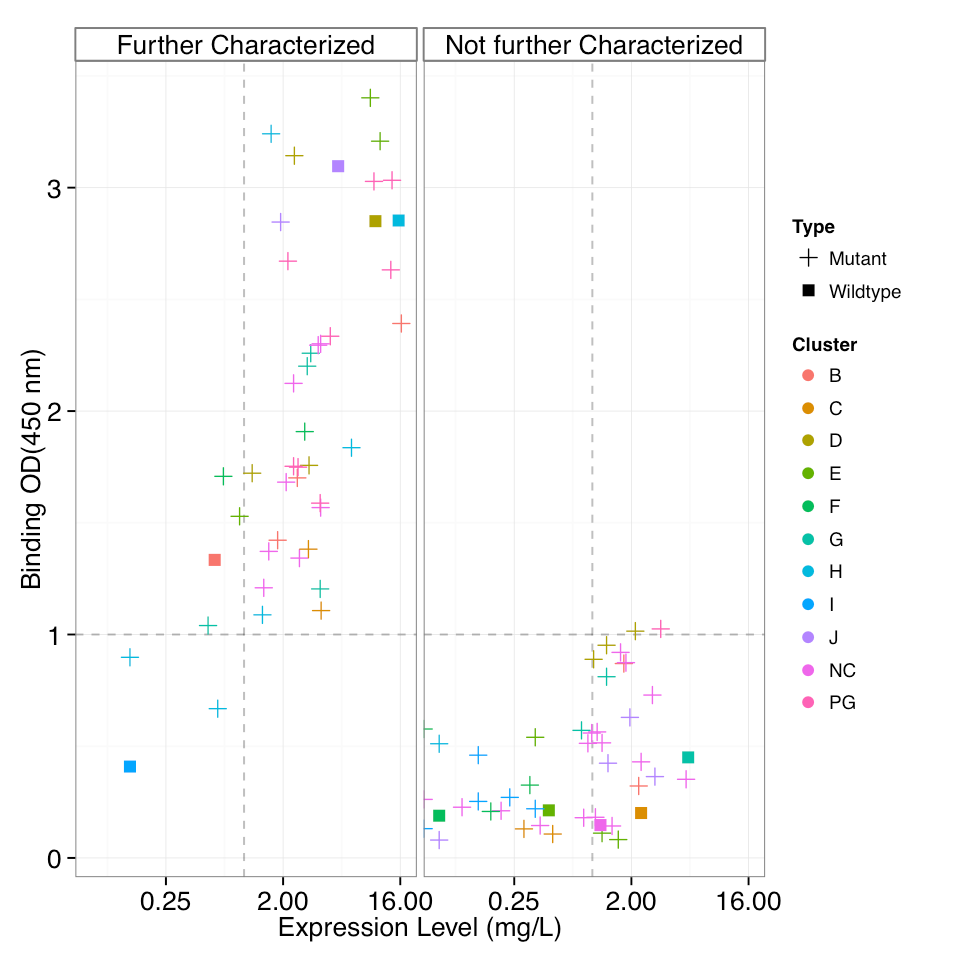
\includegraphics[width=.9\linewidth]{images/chapter3/figure3_15.pdf} % requires the graphicx package
% %    \caption[Current Sequencing Technologies]{Current sequencing technologies. On the x-axis is the current read length for each sequencing platform. The y-axis is the bases per run. Each point is a new iteration of that platforms sequencing read length and coverage. HiSeq has the most coverage with relatively short read lengths. Figure adapted from \citep{developmentinNGS:2012bs} }
% %    \label{fig:figure3_15}
% % \end{figure}

% % \begin{figure}
% %    \centering
% %    \includegraphics[width=.9\linewidth]{images/chapter3/figure3_14.pdf} % requires the graphicx package
% %    \caption[Current Sequencing Technologies]{Current sequencing technologies. On the x-axis is the current read length for each sequencing platform. The y-axis is the bases per run. Each point is a new iteration of that platforms sequencing read length and coverage. HiSeq has the most coverage with relatively short read lengths. Figure adapted from \citep{developmentinNGS:2012bs} }
% %    \label{fig:figure3_16}
% % \end{figure}


% % \begin{figure}
% %    \centering
% %    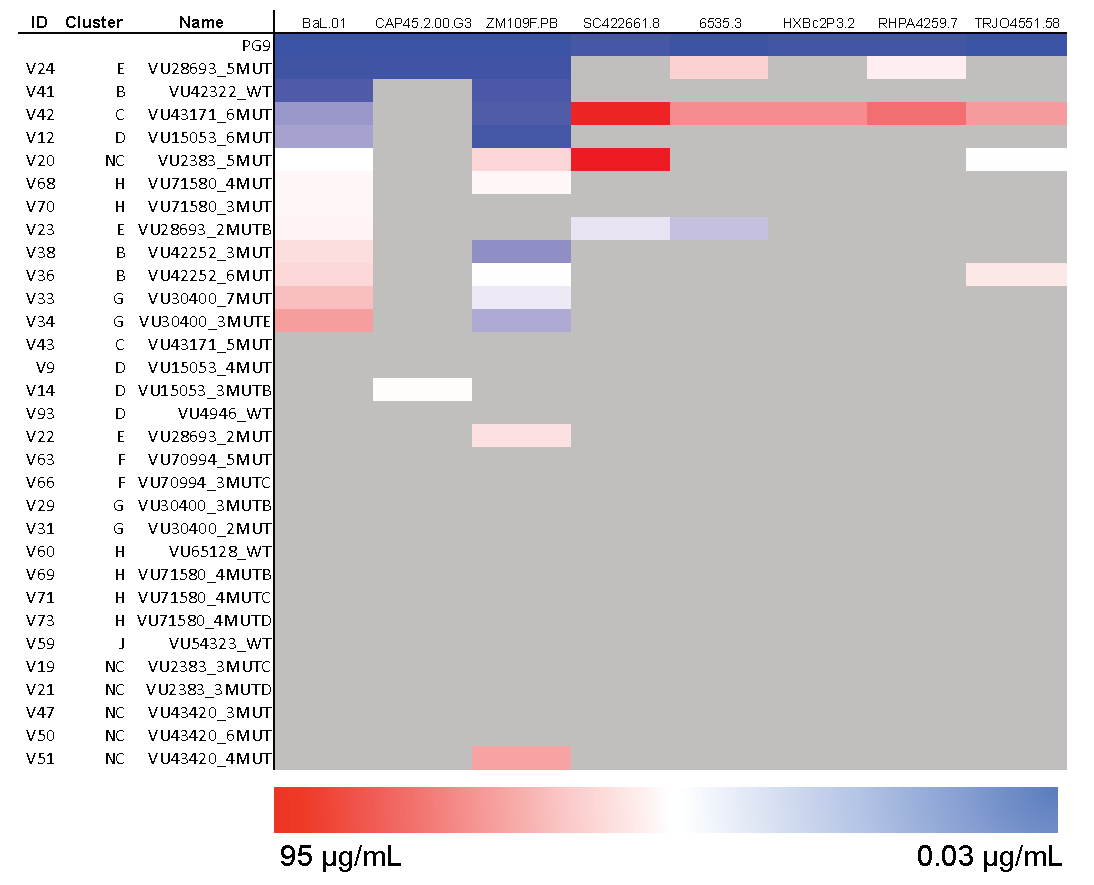
\includegraphics[width=.9\linewidth]{images/chapter3/figure3_17.pdf} % requires the graphicx package
% %    \caption[Current Sequencing Technologies]{Current sequencing technologies. On the x-axis is the current read length for each sequencing platform. The y-axis is the bases per run. Each point is a new iteration of that platforms sequencing read length and coverage. HiSeq has the most coverage with relatively short read lengths. Figure adapted from \citep{developmentinNGS:2012bs} }
% %    \label{fig:figure3_18}
% % \end{figure}

% %TABLES


% %
% %\begin{table}[!h]
\centering
\begin{tabular}{lc}
\textbf{Cluster}   & \textbf{Weighted Z-Score} \\
\hline
Cluster B & -1.24            \\
Cluster C & 0.28             \\
Cluster D & 0.11             \\
Cluster E & 0.15             \\
Cluster F & -0.34            \\
Cluster F & -0.20            \\
Cluster G & 0.31             \\
Cluster H & 0.11             \\
Cluster I & -2.54            \\
Cluster J & 1.48             \\
PG9       & -4.80            \\
PG16      & -1.87            \\
IG 4      & -1.46
\end{tabular}
\caption[Weighted Scores of PG9-Mimic Clusters]{Weighted scores of PG9-mimic clusters. The top scoring sequence for each cluster are shown with weighted the Z-score.}
\label{tab:table3_4}
\end{table}
% %\begin{sidewaystable}
\centering
\resizebox{.99\linewidth}{!}{
\begin{tabular}{cccccc}
\toprule
\textbf{Cluster} & \textbf{Total Candidates} & \textbf{Wild-Type Expressed$^{1}$} & \textbf{Mutants Expressed$^{2}$} & \textbf{Wild-Type Bound$^{3}$} & \textbf{Mutants Bound$^{4}$} \\ \hline
B                & 6                         & +                             & 5/5                         & ++                        & 3/5                     \\
C                & 5                         & ++                            & 3/4                         & -                         & 2/3                     \\
D                & 7                         & +++                           & 6/6                         & +++                       & 4/6                     \\
E                & 7                         & -                             & 6/6                         & N/A                       & 3/6                     \\
F                & 6                         & -                             & 2/5                         & N/A                       & 2/2                     \\
G                & 8                         & +++                           & 7/7                         & -                         & 4/7                     \\
H                & 7                         & +++                           & 4/6                         & +++                       & 4/4                     \\
I                & 6                         & -                             & 0/5                         & N/A                       & 0/0                     \\
J                & 6                         & +++                           & 4/5                         & +++                       & 1/4                     \\
IG               & 26                        & +                             & 23/25                       & -                         & 8/23                    \\ \hline\hline
\textbf{Total}   & \textbf{84}               & \textbf{7/10}                 & \textbf{60/74}              & \textbf{4/7}              & \textbf{31/60}         
\end{tabular}}
\captionsetup{singlelinecheck=off}
\caption[Expression and Binding Statistics]{Expression and binding statistics. Each cluster is shown with it's total number of candidates that we attempted expression and binding. We record if the wild-type sequence expressed and bound, as well as the number of mutant sequences that expressed and bound.
\begin{description}
		\item[Wild-type expression$^{1}$]: +-> 300 $\mu$g/L, ++ - > 1 mg/L, +++ - > 5 mg/L
		\item[Number of expressed mutants$^{2}$]. Positive if they expressed > 300 $\mu$g/L
		\item[Wildtype binding$^{3}$]: + -> 1 OD, ++ -> 2OD, +++ - > 3OD
		\item[Mutants bound$^{4}$]: Positive if OD > 1.0
\end{description}}
\label{tab:table3_5}
\end{sidewaystable}